\chapter{Autonomic VPNs}
\label{vpns}
In distributed computing, there are many applications for VPNs, two such tasks
are the connecting large sets of remote resources and accessing a central
server or a personal resource.  Similar use cases can be extrapolated onto
other collaborative environments such as multiplayer games, merging home
networks over a VPN, or accessing a work computer remotely.  Each application
has different requirements and in review of related research~\cite{ipop, vine,
violin, vnet, ocala, softudc, openvpn, hamachi, wippien, gbridge, pvc, tinc,
n2n, p2pvpn, l2tp} not a single approach efficiently supports these dynamic
environments.  Certainly ISP large scale VPNs such as MPLS~\cite{mpls} do not
as well.  An overview of these and the one described in this proposal are
presented in Table~\ref{tab:virtual_networks}

The organization of a VPN has a direct effect on the amount of user effort
required to connect multiple sites.  In this regard there are two components of
a VPN, the local organization and the remote or network organization.  The setup
of the virtual network in order to have be a destination and recognized source
for remote packets constitute the local organization.  Whereas the routing of
the packets amongst peers is handled by the network organization.  Prior
research works primarily focused on the latter issue, while ignoring the former.
This meant that users were left to setup their own address allocations either
through manually configuring each environment or dealing with the head aches of
caused by DHCP servers in cross domain network construction as well as their
own security distribution systems.  In addition, organizing a network can be an
even more complicated task than locally configuring the network.  This chapter
presents a novel approach to VPNs that achieves both local and network
self-configuration.

\section{Network Configuration}
The key to communicating in a VPN is creating links to the VPN and finding
the peer in the VPN.  The different architectures for VPN link creation are
based on distributed computing communication methods and are described in
Table~\ref{tab:vpn_types}.  The approaches are described in more detail
below.

\subsection{Centralized VPN Systems}
OpenVPN is an open and well-documented platform for deploying centralized VPNs.
In this paper, it is used as the basis for understanding centralized VPNs as it
represents features common to most centralized VPNs.

In centralized VPN systems, clients forward all VPN related packets to the
server.  Client responsibilities are limited to configuring the VN device and
authenticating with the VPN server; whereas the servers are responsible for
authentication and routing between clients and providing access to the servers'
local resources and the Internet (full tunnel).  Likewise, broadcast and
multicast packets also must pass through the central server.

Centralized VPNs can support multiple servers: upon starting, the client can
randomly select from a list of known servers, implementing a simple load
balance.  Once connected, the servers provide the client an IP address in the
VPN address space. Depending on configuration this will allow a client to
communicate with other clients, resources on the server's network,
or Internet hosts via the VPN.  Servers require additional configuration to
communicate with each other.

All inter-client communication flows through a central server.  By default, a
client encrypts a packet and sends it to the server.  Upon receiving the packet,
the server decrypts it, determines where to relay it, encrypts it, and then
sends the packet to its destination.  This model allows a server to eavesdrop on
communication.  While a second layer of encryption is possible through a shared
secret, it requires out-of-band communication and increases the computing
overhead on communication.


\subsection{Centralized P2P VPN Systems}
Hamachi~\cite{hamachi} is the first well-known centralized VPN that used the
ambiguous moniker ``P2P VPN''.  In reality, these systems are better classified
as centralized VPN servers with P2P links.  Similar VPNs include
Wippien~\cite{wippien}, Gbridge~\cite{gbridge}, PVC~\cite{pvc}, and
P2PVPN\footnote{Due to the similarities between the name P2PVPN and focus of
this paper, ``P2PVPN'' refers to ~\cite{p2pvpn} and ``P2P VPN'' to to the use
of P2P in VPNs.}~\cite{p2pvpn}.  The P2P in these systems is limited to direct
connectivity between clients orchestrated through a central server: in Wippien
it is a chat server, while P2PVPN uses a BitTorrent tracker.  If NAT traversal
or firewalls prevent direct connectivity, the central server can act as a
relay.  Each approach uses their own security protocols with most using a
server to verify the authenticity and setup secure connections between clients.
In regards to the P2PVPN, long term goals involve the creation of an
unstructured, which would provide a method of decentralized organization.

\subsection{Decentralized VPN Systems}
Some examples of systems that assist in distributing load in VPN systems are
tinc~\cite{tinc}, CloudVPN~\cite{cloudvpn}, ViNe~\cite{vine}, VNET~\cite{vnet},
and Violin~\cite{violin}.  These systems are not autonomic and require explicit
specification of links between resources.  This means that, like OpenVPN, these
systems can suffer VPN outages when nodes go offline, thus administrators must
maintain the VPN connection table.  Unlike OpenVPN, these approaches typically
do not require all-to-all direct connectivity for all-to-all communication.
Users can either setup out-of-band NAT traversal or route through relays.  Links
are manually configured.

\subsection{Unstructured P2P VPN Systems}
Unlike centralized and decentralized systems, P2P environments require the
user to connect to the overlay, which then automatically configures links.
The simplest form of overlays are unstructured, where peers form random
connections with each other and use broadcast and stochastic techniques to find
information and other peers, though due to its unstructured nature, the system
cannot guarantee distance and routability between peers.  The only example of
an unstructured VPN is N2N~\cite{n2n}.  In N2N, peers first connect to a super
node and then, to find another peer, they broadcast discovery messages to the
entire overlay.  In the case that peers cannot form direct connection, peers
can route to each other over the N2N overlay.  In the realm of VPNs, all client
VPNs are also servers performing authentication though neither approach deals
with decentralized address allocation.

\subsection{Structured P2P VPN Systems}
To address the scalability concerns in unstructured systems, this work uses
structured P2P overlays.  As described in Chapter~\ref{structured_p2p},
structured P2P overlays provide distributed look up services with guaranteed
search time with a lower bound of $O(\log N)$, in contrast to unstructured
systems, which rely on global knowledge/broadcasts, or stochastic techniques
such as random walks.  In general, structured systems are able to make these
guarantees by self-organizing a structured topology, such as a 2D ring or a
hypercube, deterministically by randomly generated node identifiers.

The primary feature used by structured overlays is a distributed data store
known as a distribute hash table (DHT), which stores key, value pairs.  In
the overlay, the key is an overlay address, where the value is stored.  The
peer closest to the key's overlay address is responsible for maintaining the
value.  Cryptographic hashes like SHA and MD5 can be used to obtain the key's
overlay address from a string or some other byte array.

In~\cite{pcgrid07, i3}, a method for address allocation is described by using
the DHT.  Each VPN has a unique name or namespace, when a peer requests an
IP address, a mapping of $hash(namespace, IP)$ to the peers overlay address
is atomically written to the DHT.  A success implies that the writer was the
first writer to that value and other peers reading that value will be able to
identify that peer as owner of that IP address in that namespace.  Likewise
when a peer wants to route a packet to a remote VPN peer, they query the DHT
using the mapping, which returns the overlay address.  The IP packet is then
sent to the overlay destination.

Unicast messages are sent between two end points on the overlay using normal
overlay routing mechanisms.  Direct overlay links can be used to improve
performance between end points.  ~\cite{ipop} describes a method by which peers
can form autonomic direct connections with each other using an unstructured
overlay.  As IP traffic increases over a period of time, a direct connection to
bypass the overlay is initiated by the receiver of the packets.  Alternatively,
a VPN may wish to form all-to-all connections with VPN peers as described
in~\cite{cops08}.

To support broadcast and multicast in an overlay, all members of a subnet
associate through the DHT by placing their overlay address at a specific key,
i.e., $namespace:broadcast$.  Then when such a packet is received, it is sent
to all addresses associated with that key.  It is up to the VN at each site to
filter the packet.  This is sufficient to support deployments where multicast
or broadcast is not relied upon extensively.  

\section{Local Configuration}
From a superficial point of view there are two approaches to local VPN
configuration a single VN endpoint per a host (Interface) and a VN router
endpoint for many hosts on the same LAN (Router).  The components differing
between the two approaches are:
\begin{itemize}
\item \textbf{Software location} - Interfaces execute the software on each VPN
connected resource, whereas any machine connected to the same LAN as a Router
will be able to access the VPN.  The Router requires a dedicated resource.
\item \textbf{Network configuration} - Since the Interface software runs on
each machine, it is able to directly configure networking parameters, whereas a
Router must use external methods to configure the resources.
\item \textbf{Communication on a LAN} - When two peers on a LAN using a VPN
Interface to communicate, all traffic must pass through the VPN adding
unnecessary overhead, though in a Router the two peers have a merged physical
and virtual network between them and the traffic is able to bypass the VPN.
\item \textbf{Fault tolerance} - The Router only has a single instance running,
when it goes offline, all resources will lose their VPN access, whereas each
individual resource has their own Interface and is responsible for their own
VPN connectivity.
\item \textbf{Communication over the WAN} - Performing encryption can be
expensive and may limit the bandwidth available due to CPU constraints.  A
Router may struggle to use all the available bandwidth, whereas enough
Interfaces will eventually be able to use all the bandwidth.  Although each
additional VPN Interface also has idle traffic, potentially reducing usable
bandwidth.
\end{itemize}

This proposal identifies methods by which a single software stack can be
implemented to support self-configuration and resource migration in a way that
is platform independent.  This method lends itself to a new architecture known
as Hybrid, allowing an instance to be run on each VPN resource but enabling
direct communication amongst peers on a LAN as described in~\cite{sc09}.  The
architectures are shown communicating via an overlay in
Figure~\ref{fig:three_models} and compared in Table~\ref{tab:three_models}.
The two aspects that need configuration in the local configuration beyond the
VPN architecture are address allocation, obtaining and setting an IP address on
a resource, and address resolution, determining where to route a VPN packet.
The keys to creating this environment involve the use of standard network
protocols implemented uniformly across operating systems, including DHCP
(dynamic host configuration protocol) and ARP (address resolution protocol).
Many applications make use of names instead of IP addresses to resolve peers,
as such a naming system, like DNS (domain name service) is almost as important
as address resolution and allocation.  A state machine representation of this
architecture is shown in
Figure~\ref{fig:vn}.

\subsection{Local VPN Architecture}
As described in the introduction, the TAP device is the glue by which the local
resources communicate with the VPN.  Each approach relies on the TAP device
though in different configurations.  In the Interface
(Figure~\ref{fig:interface}), the TAP device is used directly by the user as
any other network device.  In short, packets are written to the TAP device by
the O/S sockets and read by the VPN software to send to the remote location,
packets received by the VPN are written to the TAP device and delivered to
sockets by the O/S.  The Router (Figure~\ref{fig:router}) bridges the TAP
device to a LAN, thus packets can be routed to it and sent through the VPN.
TAP device virtualizes a bridge to other physical networks.  

Finally, the Hybrid (Figure~\ref{fig:hybrid}) like the Router connects to the
LAN but only allows configuration from the local host.  In Linux this is
possible through the use of a VETH pseudo device that provides a virtual
Ethernet pair, so that one end can be bridged with the TAP device and LAN while
the other provides another interface that can be configured on the LAN, which
will be used by the VPN.  The reason for this lies in the nature of the state
of the interfaces connected to the bridge, which go into promiscuous mode, so
that all packets sent to them are forwarded on as if they are on a wire as if
there were only a single network interface.  In non-promiscuous mode, the
network card will drop packets that are not destined for that network card.
So in that case, it is not possible to assign more than one IP address to a
bridge, because it and all devices connected to it are viewed as one big network
interface.  Connecting the VETH device allows an additional uniquely
identifiable Ethernet addresses and thus additional IP addresses.  In contrast,
aliasing a Ethernet card only provide additional IP addresses and services that
rely on layer 2 networking. In this case, some services may not work, for
example, DHCP does not work on aliased network cards.

\subsection{Address Resolution}
IP is a layer 3 protocol. Layer 2 devices such as switches, bridges, and hubs 
are not aware of IP addresses.  When a system wants to send a layer 3 packet
over a layer 2 network, it first uses ARP to find the layer 2 address owning
the layer 3 address.  This process, as shown in Figure~\ref{fig:arp}, begins by
the sending of a layer 2 broadcast message which contains an ARP request,
asking all members in the LAN that the node owning the target IP address
respond to the sender of the request.  If a node owns the target IP address,
it responds with an ARP reply, making themselves the sender and the original
sender is the message recipient.  The Ethernet header consists of the source
address being the sender and the target being the destination.  By listening to
these requests, layer 2 devices such as a switch can autonomously learn the
location of nodes holding Ethernet addresses are and can forward packets
through appropriate ports as opposed to broadcasting or dropping them.

In a typical IP subnet, all machines talk directly with each other through
switches.  As such, they must learn each other's Ethernet address. The VN model
used in this proposal focuses on a large, flat subnet spanning across all nodes
connected to the VPN.  To accomplish this, the VN provides the ability to
virtualize a bridge, similar to proxy ARPs~\cite{RFC0925} used to implement a
transparent subnet gateway~\cite{RFC1027}.  In this scenario, the VN would
need to respond to the ARP packets with a fake layer 2 address.  Layer 2
devices in the system would then route all packets destined for that layer 2
address to the VN.

As shown in the state machine (Figure\ref{fig:vn}), ARPs are only responded to
if (a) they are inquiring about a VN IP address, (b) the VN address is not
locally allocated, and (c) there is a P2P:IP mapping.  If all those are true,
then an ARP response is sent back to the sender.  ARPs are occasionally sent
out during the course of communication and thus if a machine migrates to a VN
router, the VN router will no longer respond with ARPs.  An ARP response sent
by the VN requires a source Ethernet address, bridges and switches will see the
response and will forward all traffic towards the TAP device for that Ethernet
address.  A VN device can use the same Ethernet address for remote entities.

Prior to the introduction of the VN hybrid, the VNs used the Ethernet address
FE:FD:00:00:00:00 to refer to remote entities.  If each VN hybrid used this
address, there would be layer 2 collision causing a single hybrid to have all
traffic sent to it.  In hybrid mode, each VN must generate a unique ``remote''
Ethernet address at run time.  Experience and research has led to the
following solution: (1) use FE:FD for the first two bytes as they tend to be
unallocated and (2) assign random values to the 4 remaining bytes.   Applying
the birthday problem in this context, the expected probability of address
collisions is small for typical LAN environments (less than 50\% if the average
number of VN hybrid nodes on the same L2 network is 65,000). 

The key difference from the Hybrid and Router is that the Hybrid routes for only
a single node, say ``A'', and thus must ignore messages that do not originate
from ``A''.  The Hybrid model does not necessarily know about the existence of
all machines in a LAN, because it does not own them.  So when an ARP request
of some remote machine, say ``B'', is sent by ``A'', the Hybrid must send out
a matching request with the result being sent back to the pseudo-entity of the
transparent subnet gateway so that the VPN can determine if ``B'' exists
locally.  If no message is returned after a set amount of time (the reference
implementation used 2 seconds), then assuming that there is a peer in the
overlay with the IP address, the original ARP will be responded to with the
pseudo-entity being the target.

\subsection{Address Allocation}
IP addresses are traditionally allocated in one of three ways: 1) statically, 2)
dynamically through DHCP, or 3) through pseudo-random link-local addressing.
This model focuses on static and dynamic addressing.

The network components configurable by DHCP as defined by~\cite{dhcp0,dhcp1}
that are interesting to a VPN are addresses, routing, and other networking
related features.  While many different client and servers exist, they all tend
to support the basic features of allowing the server to specify to a client and
IP address, a gateway address, and domain name servers.  As shown in
Figure~\ref{fig:dhcp}, the steps in DHCP are:
\begin{enumerate}
\small{
\setlength{\itemsep}{0pt}
\setlength{\parskip}{0pt}
\item Client sends Discover packet requesting address.
\item Server receives the packet, allocates an address, and sends an Offer of
the address and other network configuration.
\item Client receives and acknowledges the Offer by sending a Request message
to accept the Offer.
\item Server receives Request message and returns an ACK message containing
the same details as the Offer.
}
\end{enumerate}

During the DHCP phase, the VPN communicates with a DHCP server for the VPN,
which will allocate an address for the requester.  Similarly, a VN model can
review packets coming into the VPN, review the sender IP address, and request
and notify the server of this allocation.  Treating static addresses like
DHCP enables easier configuration of the VPN, though it is difficult to handle
address conflicts.  In this model, this is done by the server ignoring the
duplicate requests, and it is up to the user to configure for a new address.
Thus DHCP provides a more reliable method in these systems.

To support scalable address allocation in decentralized systems, the
DHCP server is a virtual entity, parsing DHCP packets and interacting with
an overlay based DHT.  This approach does not need to be limited to structured
overlay based VPNs but can be introduced as an added value component.

An important aspect of DHCP is that after a machine has received an IP address
from the DHCP server, it always checks to ensure that the address has not been
allocated, as such the VPN should never respond to address resolutions for
local IP addresses.

If an overlay allocates an address to the VN, then the VN owns it.  The other
address that the VN owns is the null address, 0.0.0.0, which is sent during
DHCP to indicate that the machine has no address prior to the request.

\subsection{Domain Name Servers and Services}
Name services allow machines to be addressed with names that are more
meaningful to users than numeric addresses.  Certain applications and
services require domain name checking, such as Condor.  To support DNS, this
requires that the OS be programmed with the VN's DNS servers IP, typically
the lowest available IP address in a subnet.  In static configuration, this
process requires the user to manually add this address, though through DHCP
this is set automatically.

In the state representation of the VN (Figure~\ref{fig:vn}), the VN checks the
IP packet to ensure that the destination IP and port match that of the virtual
DNS server and the well-known DNS port, 53.  In the event of a match, the
packet is passed to the VN's handler for domain names.  Names are typically
used for the following purposes: 1) because applications require it, and 2) to
assist users in finding resources.  To deal with 1), the DNS can
deterministically maps IP addresses to names, such as 10.250.5.5 maps to
C250005005.  2) can be solved by using the DHT and placing key:value pairs of
the form hash(namespace:hostname) to IP address and hash(namespace:IP address)
to hostname.

\section{Socket and HTTP Proxy VPNs}
\label{userspace_vpn}
In certain circumstances, users are unable to run their own VPN software
limiting their ability to connect with other resources through specialized tools
like Smart Sockets~\cite{smartsockets} or manually created links.  Neither of
these approaches allow direct communication to resources already connected to
a VPN without additionally adding support for more features.  To address this
issue, I propose the implementation of an entire networking stack in software
from the transport layer, including TCP, UDP, and ICMP, down to the data
link layer, as to include IP and Ethernet.

Methods that enable connecting to a user space VPN include HTTP/Socks proxy,
sockets API, or port redirection.  The proxy methods requires that the client
application support redirecting traffic to the HTTP/Socks proxy.  The sockets
API will require that the application be recompiled using a different sockets
API than the one shipped with the host, providing a challenge for programming
language transparency.  Port redirection works by telling the local application
that the program is running on a local IP address and port, but the VPN
application runs at that location, encapsulates the packet through the user
space VPN stack, and forwards the packet via the overlay to the remote peer.
Much of the ground work for a user space VPN has been set, as IPOP naively
supports the physical layer, has an understanding of Ethernet and IP
communication, and supports parsing and creating Ethernet, ARP, IP, TCP, ICMP,
UDP, DHCP, and DNS packets.  The remaining components are the TCP stack, which
will be completed by the work done in Chapter~\ref{tcp}, a userspace Ethernet
and IP system, ICMP and UDP handlers, and the HTTP proxy and socket bindings.

The usefulness of this work will be verified in high performance environments
and supporting web servers.  The experiment involving high performance
computing lab resources, where users do not have the ability to run
privileged applications, will explore how quickly resources can be added to a
a Condor pool.  A challenge in supporting the group systems in private overlays
is lack of ability to host a website.  Using this method a website can be hosted
non-obtrusively over a VPN.

\section{Supporting Migration}
There has been a rapid increase in the deployment of Virtual Machines (VMs) for
use in resource consolidation in the server industry as well as the domain of
cloud computing.  Providers of cloud computing services have adopted virtual
machines as the unit of granularity for providing services and service level
agreement to the users.  Users are billed according to the number of VMs and
their uptime. Major cloud-computing providers including Amazon EC2 and Go-Grid
have adopted Xen as the virtualization platform for their services and sell
compute resources in the form of virtual machines.

Apart from advantages like performance isolation, security, and portability, one
of the significant advantages of using VMs is the capability to migrate the VM
with its entire software stack from one physical host to another.  This
migration may be performed in a stop-restart manner, where the VM is paused,
migrated to another host and restarted, or in a live mode, which attempts to
minimize down time to reduce interruption of services running on the VM.

VMs including Xen~\cite{xen-live}, VMware ESX~\cite{vmotion} and KVM~\cite{kvm}
support migration with two critical requirements: (1) file systems (disk images)
must be on a shared storage system (i.e. network file systems or storage area
networks) and (2) to maintain network connectivity, the migration must occur
within an IP subnet.  In order to retain network connectivity after migration,
the VMM must notify the LAN of the VM's new location.  The new VMM host
generates an unsolicited ARP reply which broadcasts to the entire network the
VM's new location.  

The VN Interface and Hybrid models support migration of the virtual address
using techniques previously described in~\cite{ipop}.  This is a product of the
decentralized, isolated overlay approach where each overlay end point has a
one-to-one mapping to VN end point, e.g., P2P to IP.  When a VN Interface or
Hybrid model migrates, the overlay software must reconnect to the overlay, at
which point, packets will begin to be routed to the VN endpoint again,
completing migration.

Unlike Interface and Hybrid models, the VN Router does not support a one-to-one
mapping.  In fact, a VN router tends to have one P2P address for many IP
addresses.  When a machine with a VN IP wants to migrate, it cannot also take
its P2P address with it otherwise it would end connectivity for the rest of the
members of the VN router shared  overlay end point.  A solution to this
problems requires the ability to delete IP-to-P2P mappings in the DHT, detect
new addresses on the network, and inform senders that an IP is
no longer located at that overlay end point.  With these capabilities,
transparent migration can be achieved for the VN router model as follows. 

The VMM initiates a migration on a source node. Until the migration completes,
the VN router at the source continues to route virtual IP packets for the
VM. Upon completion of migration, the VN router at the target learns about
the presence of the migrated VM by either receipt of an unsolicited ARP
or by proactively issuing periodic broadcast ICMP messages on its LAN.
The VN router attempts to store (Put) the IP:P2P address mapping in the DHT,
and queries for the existence of other IP:P2P mapping(s). If no previous
mappings are found, the VN router assumes responsibility for the IP
address. Otherwise, the VN router sends a migration request to each P2P
address returned by the DHT. The VN router receiving a migration request
confirms the existence of the IP address in its routing table and that if
there is that there is no response to ARP requests sent to the IP address.
If these conditions hold, it deletes its IP:P2P mapping from the DHT and returns
true to the migration request; otherwise, it returns false. If the migration
request returns true, the VN router at the target LAN starts routing for the
virtual IP address; if it returns, false, the VN router does not route
for the virtual IP address until the previous IP:P2P mapping expires
from the DHT.

In addition to VN routers synchronizing ownership of the migrated virtual
IP address, any host that is connected to that machine must be informed
of the new P2P host.  Over time, this will happen naturally as ARP cache
entries expire and the IP:P2P mapping is looked up from the DHT.  Additionally,
the VN router at the source may keep forwarding rules for the migrated IP
address for a certain period of time, akin to mobile IP but not on a permanent
basis.  A more direct approach, as implemented in the prototype, involves the VN
router notifying the connected host of a change in ownership, resulting in the
host querying the DHT for the updated P2P end point.  An evaluation of trade offs
in the migration design, while interesting, is outside the scope of this paper. 

A static address allocation is similar to a migration without there being an
IP:P2P value in the DHT, though without querying the DHT, the situation is
unclear.  Systems that use DHCP only must have some method for detecting new
addresses, because there is no guarantee that a DHCP will occur immediately
following migration, in fact, depending on the lease time that is highly
unlikely.  Using an insecure DHT that supports deletes is sketchy as it would
be relatively easy for machines to perform man in the middle attacks by
deleting keys which they do not own.  Even the use of passwords mentioned in
DHT literature is not sufficient as it is not immune to collusion, or Sybil,
attacks.

VN router migration was analyzed through the use of two Xen-based VMware VMs
co-located on the same quad-core Xeon 5335 2 GHz machine each with 1 GB memory
allocated using a minimally configured OS with a SSH server.  The evaluation
attempts to understand overlay overheads of the approach.  The experiment, as
shown in Figure~\ref{fig:migration_ring}, involved migrating a Xen guest VM
between two Xen host VMMs running in VMware.  Although they are hosted in the
same infrastructure, the two domains are connected to two separate VLANs, and
thus isolated.  The resource information is stored in a DHT running on top of
PlanetLab.  Thus the migration overheads in the experiment capture the cost of
wide-area messaging in a realistic environment.  During the course of the
experiment, over 50 different IP addresses were migrated 10 times each in an
attempt to gain some insights in the cost of using the DHT with support for
deletes and VN router messages as a means to implement migration.  The result,
presented in Figure~\ref{fig:mig} gathered from the experiment was how long the
VN IP was offline, measured by means of ICMP ping packets.  On average, the
overhead of VN migration was 20 seconds. This overhead is in addition to the
time taken to migrate a VM, since the VN routers begin to communicate only
after migration finishes. 

\section{Enhancing the Structured P2P VN with Private Virtual Overlays}
The use of group enabled private virtual overlays enable two qualities for
VPN:  user-friendly security and more efficient methods for broadcast and
multicast IP communication.

\subsection{Securing the VPN Through Groups}
\label{groupvpn}
The premise for secure a structured overlay VPN extends from the work on
group enabled private virtual overlays.  Each VPN will use a unique private
overlay secured by a group-enabled PKI.  For VPN purposes, both the overlay
control messages are encrypted as well as IP traffic, protecting the overlay
from malicious third-parties but all the IP traffic between two members from
other members.

The group overlay model requires a few modifications to be applied to a group
VPN.  During the creation of the group, the administrator configures the VPNs
address range, namespace, enabling security, and if they would like to use an
existing public overlay network or provide their own set of overlay nodes.
When a user has been accepted into the group, they are able to download VPN
configuration data, which is used to self-configure the VPN.  The configuration
is self-contained and requires that the user provide it to the VPN, by either
placing it in a specific directory, a GUI, or a command-line utility whose only
input parameter is the path to a configuration file.  In the prototype, the
only the file system and command-line approaches have been implemented.  The
configuration data contains the IP address space, VPN namespace, group web site's
address, and a shared secret.  The shared secret uniquely identifies the user,
so that the website can determine how to handle certificate requests.  When
making a certificate request, the user sends over HTTPS a public key and their
shared secret, the website creates and signs a certificate request based upon
the public key and the user's relevant information ensuring that users cannot
trick the website into signing malicious data.  Upon receiving the signed
certificate, peers are able to join the private overlay and VPN enabling
secure communication amongst the VPN peers.

\subsection{Broadcasting IP Broadcast and Multicast Packets Via the Overlay}
The use of a private virtual overlay enables a new method for sending multicast
and broadcast packets. Approaches such as broadcasting to the entire overlay
are not suitable because the overlay could consist of peers from other VPNs and
those not even involved with VPN operations, while approaches that generate
unicast messages when a broadcast or multicast packet arrives at the VPN (e.g.
by querying a DHT key where all peers in the VPN would place their overlay
address so that they could receive the packets) do not scale well. The
abstraction of a private virtual overlay enables scalable broadcasting within a
VPN because the only peers in the private overlay are peers for a single VPN.
The broadcast method used is described in Appendix~\ref{broadcast} to
efficiently distribute messages.  Though in VPN situations, many peers may
already have connections to most if not all of their VPN peers, thus the
broadcast algorithm has been modified to route to only connections created for
structured overlay purposes and not explicitly only for VPN purposes.
Otherwise in many cases, this algorithm will degenerate into one similar to
the previous approach.  

A validation of the overlay broadcast method for IP broadcast and multicast
communication comparing it to the original DHT method is presented in
Figure~\ref{fig:broadcast}.  Metrics measured include bandwidth used by
the packet originator and time required for all peers to receive the packet.
System bandwidth remains the same as bounded-broadcast requires exactly N
messages to broadcast the message to the entire overlay.  By using a broadcast
algorithm to route multicast and broadcast IP packets instead of the unicast
packets, the sending node has much less used bandwidth.  The time required by
the DHT approach involves the time to retrieve all entries from the DHT and the
latency to the peer farthest away.  Whereas the broadcast approach has no DHT
lookup and is somewhere around the average latency in the system multiplied by
$O(\log^2 N)$.

\section{Full Tunnel VPN Operations}
\label{full_tunnel}
The configuration detailed so far describes a split tunnel: a VPN connection
that handles \emph{internal VPN traffic only, not Internet traffic}.  Prior
to this work, only centralized VPNs currently support full tunnel: providing
the features of a split tunnel in addition to securely forwarding
\emph{all their Internet traffic} through a VPN gateway.  A full tunnel provides
network-layer privacy when a user is in a remote, insecure location such as an
open wireless network at a coffee shop by securely relaying all Internet traffic
through a trusted third party, the VPN gateway.  Both models are illustrated
in Figure~\ref{fig:tunnel}.

Central VPN clients use full tunneling through a routing rule swap, setting
the default gateway to be an endpoint in the VPN subnet and traffic for the
VPN server is routed explicitly to the LAN gateway.  This rule swap causes
all Internet packets to be routed to the VN device and the VPN software
can then send them to the remote VPN gateway.  At the VPN gateway, the packet
is decrypted and delivered to the Internet.  A P2P system encounters two
challenges in supporting full tunnels:  1) P2P traffic must not be routed
to the VPN gateway and 2) there may be more than one VPN gateway.  We address
these issues and provide a solution to this problem in Section~\ref{full_tunnel}.

The challenges faced in a decentralized P2P VPN are providing decentralized
discovery of a VPN gateway and supporting full tunnel mode in a P2P environment
such that all P2P traffic is sent to the intended receiver directly instead of
through the gateway.  The remainder of this section covers gateway and
client solutions to address these challenges.

\subsection{The Gateway}
\label{the_gateway}
A gateway can be configured through NAT software, like masquerading in IPtables
or Internet Connection Sharing with Windows.  This automatically handles the
forwarding of packets received on the NAT interface to another interface
bringing the packet closer to its destination.  Similarly, incoming packets
on the outgoing interface must be parsed in order to determine the destination
NAT client.

Following from the original design of the VPN state machine in
Figure~\ref{fig:vn}, if a VPN is a gateway, the VPN state machine no longer
rejects packets, when the destination is not in the VPN subnet, though when the
VPN gateway mode is disabled these packets are still rejected.  When enabled,
all Internet and non-VPN based traffic is written to the TAP device setting the
destination Ethernet address to the TAP device.  The remaining configuration is
identical to other members of the system as packets from the Internet will
automatically have the clients IP as the destination as a product of the NAT.
To provide for dynamic, self-configuring systems, VPN gateways announce their
availability via an entry in the DHT.  As future work, this approach can be
explored to provide intelligent selection and load balancing of gateways.

\subsection{The Client}
VPN Clients wishing to use full tunnel must redirect their default traffic to
their VN device.  In the prototype VPN model, a virtual IP address is allocated
for the purpose of providing distributed VN services DHCP and DNS.  This same
address is used as the the default gateway's IP.  Because this IP address never
appears in a Internet bound packet, only its Ethernet address does, as shown in
Figure~\ref{fig:tunnel_packet}, this approach enables the use of any and
multiple remote gateways.

To support full tunnel mode, the VPN's state machine has to be slightly modified
to handle outgoing packets destined for IP addresses outside of the VPN, only
rejecting them when full tunnel client mode is disabled.  When enabled, the VPN
software sends packets to the remote peer acting as a full tunnel gateway.
Likewise, incoming packets that have a source address outside the subnet should
not be rejected but instead the overlay address should be a certified VPN
gateway prior to forwarding the packet.

To select a remote gateway, peers query the DHT.  As there may be multiple
gateways in the system, the peer randomly selects one, forwarding packets to
that node.  To ensure reliability, when the client has not heard from the
gateway recently, the client sends a liveness query to the gateway.  If the
gateway is down, the taken pessimistic approach finds a new gateway when
the next Internet packet arrives.

The real challenge in applying full tunnel VPN mode to P2P VPNs is the nature
of the P2P system, namely dynamic connections.  Peers do not know ahead of time
what remote peer connections will be thus a simple rule switch does not work.
The original approach was to watch incoming connection requests and adding
additional routing rules on demand, though this is only reasonably feasible
with UDP as a TCP handshake message would need to be intercepted and potentially
replayed by the local host in order to enable the rule and allow proper routing.
The real drawback of the approach though is that UDP messages can easily be
spoofed by remote peers enabling unsecured Internet packets to be leaked in the
public environment.  Even if the connections are secured, it could take some
time for the peers to recognize a false connection attempt and delete the rule.

A solution to the security problem is to have all traffic directly routed to
the VN device with no additional routing rules.  The VN is then responsible for
filtering P2P traffic and forwarding it to the LAN's gateway via Ethernet
packets.  In the VPN application, outgoing IP packets' source ports are
compared to VPN application's source ports.  Upon a match, the VPN application
directs the packet to the LAN's gateway.  The three steps involved in this
process are 1) translating the source IP address to match the physical
Ethernet's IP address, 2) encapsulating the IP packet in an Ethernet packet
with a randomly source address~\cite{sc09} and the destination the LAN's
gateway, and 3) sending the packet via the physical Ethernet device.  Sending
an Ethernet packet is not trivial as Windows lacks support for this operation
and most Unix systems require administrator privilege.  An alternative, platform
independent solution uses a second TAP device bridged to the physical Ethernet
device, allowing Ethernet packets to be sent indirectly through the Ethernet
device via the TAP device.  Because the solution results in incoming packets to
arrive at a different IP address than the actual original source IP address TCP
does not work in this solution.  This method has been verified to work on both
Linux and Windows using OS dependent TAP devices and bridge utilities.

\subsection{Full Tunnel Overhead}
\label{full_tunnel_eval}
While the full tunnel client method effectively resolves the lingering problem
of ensuring that all packets in a full tunnel will be secure, it raises an
issue:  could the effect of having all packets traverse the VPN application be
prohibitively expensive.  Analysis of this approach compares it with one that
uses the traditional routing rule switch.  Figure~\ref{tab:full_tunnel_eval}
present the ping time from a residential location to one of Google's IP
addresses using a gateway located at the University of Florida when the VPN is
in split tunnel mode, full tunnel using the routing rule switch, and full
tunnel using Ethernet forwarding.  The results express that there is negligible
difference between the full tunnel approaches.  One interesting result is the
latency to gateways public address in the routing test, which most likely is a
result of the ping being sent insecurely avoiding the VPN stack completely.

\section{Evaluation of VPN Network Configuration}
This experiments explores bandwidth and latency in a distributed VPN system to
motivate the usage of P2P links in a VPN.  The VPNs used are include the
prototype (IPOP), OpenVPN, and Hamachi.  OpenVPN represents a typical
centralized VPN, while Hamachi represents a well-tuned P2P-link VPN.  The
evaluation was performed on Amazon EC2 using small instance sized
Ubuntu i386 instances to create various sized networks ranging from 1 to 32.
OpenVPN uses an additional node as the central server and Hamachi has an upper
bound of 16 due to limitations in the Linux version at the time of this
evaluation.  To perform bandwidth tests, the instances are booted and query an
NFS for the list virtual IP addresses, peers are ordered such that half the
peers are act as clients and the other half the peers creating a 1 to 1 mapping
between all sets.  Latency and bandwidth tests are performed using netperf's
request-reply and streaming tests respectively.  Prior to the start of the
tests, peers have no knowledge of each other, except the virtual IP addresses,
thus connection startup costs are included in the test.  Test are run for 10
minutes diluting the connection initiation overhead but represent an example of
real usage.  Results from the clients are polled at all locations and averaged
together, though the OpenVPN server is measured separately.  IPOP and OpenVPN
use authenticated 128-bit AES, while Hamachi does not allow configuration of
the security parameters and uses the default Hamachi settings.

Figure \ref{fig:latency} and \ref{fig:bandwidth} present the results for latency
and bandwidth respectively.  Latency is measured in transactions of successful
request/reply messages.  In the latency test, it is obvious that having the
central server increases the delay between the client and server and the results
degrade more quickly as additional peers are added to the system.  In small
systems, OpenVPN shines probably due to optimized software, though as the system
grows, the system bandwidth does not.  By the time 8 peers have entered into
the system, both decentralized approaches perform better than the OpenVPN
solution.  To summarize, decentralized VPN approaches provide better
scalability, which can be immediately noticed by low latency times and, as the
system grows, available bandwidth.

\section{Evaluation of VPN Local Configuration}
This section presents an evaluation of the different VN models, using prototype
implementations built upon IPOP.  The grid evaluation simulates a client/server
environment and investigate CPU / networking overheads related with each
approach.  In addition a cloud deployment shows a proof of concept that connects
multiple cloud and local resources as well as evaluation of overhead of the
different approaches in WAN and LAN environments.  In all WAN experiments, a
wide-area IPOP overlay network with approximately 500 overlay nodes distributed
across the world on PlanetLab resources is used to bootstrap VN connections and
to support DHT-based storage and P2P messaging.

The proposed VN models place varying demands on the resources of the systems
involved. The evaluation focuses on CPU as experience suggest that this is the
most significant limiting factor.  As will be presented, the CPU load offered
by these models depends on the bandwidth of the underlying network link, since
a larger bandwidth requires more processing of packets.  The tools for
evaluating these VN models are, Netperf and SPECjbb, described in
Appendix~\ref{evaluation_tools}.

\subsection{On the Grid}
The initial evaluation involves testing a client-server environment.  The
baseline hardware consisted of quad-core 2.3GHz 5140 Xeon with 5 GB memory and
Gigabit network connectivity.  Each VM was allocated 512 MB of RAM and ran
Debian 4.0 using a Linux 2.6.25 kernel.  The client side consisted of 4 VMs on
5 machines.  The server side consisted of 5 VMs on one machine with 4 acting
as servers and 1 acting as a gateway, which was necessary to control bandwidth
into the system, done through the Linux utility \textbf{tc}~\cite{tc}, traffic
control.  In this environment, each server had 5 clients communicating with it.
The setup is shown in Figure~\ref{fig:gridsetup}.

The evaluation results are presented in Figure~\ref{fig:gridevalnet} and
\ref{fig:gridevalcpu}.  The maximum bandwidth of 600 Mbps is achieved when
neither virtual network nor traffic shaping are enabled (``no spec.phys'' at
1000 Mbps limit in Figure~\ref{fig:gridevalnet}\subref{fig:stream.netperf}),
which is only 60\% of the theoretical maximum.  This limit is most likely the
cost of VMMs, specifically the time required for a packet to traverse both VMMs
networking stack as well as the hosts networking stack.  Another observation
was that transactions per second (Figure~\ref{fig:gridevalcpu}
\subref{fig:rr.spec}) do not improve significantly for \textbf{tc} bandwidth
limit above 25 Mbps in all cases; thus focus is on only the relevant data up to
this limit.

Distinguishing features of the different VN models include the following.
Figure~\ref{fig:gridevalnet}\subref{fig:stream.netperf} shows that bandwidth in
all VN models is comparable with traffic control limit up to 75 Mbps. Beyond
this point, the interface model achieves better bandwidth than the router model
(VN processing is distributed across multiple processes); the spec/no spec
ratio in the router model is smaller than in the interface model because there
is less resource contention caused by VN processing on end nodes. For the same
reason, the router tends to achieve better SPEC results
(Figure~\ref{fig:gridevalcpu}\subref{fig:stream.spec}) than the interface.
Figure~\ref{fig:gridevalnet}\subref{fig:rr.netperf} shows that the router
performs poorly compared to the interface model in terms of
transactions/second, though it achieves a better ratio of SPECjbb score
(Figure~\ref{fig:gridevalcpu}\subref{fig:rr.spec}) to transactions than the 
interface at constrained bandwidths (less than 5 Mbps).

The hybrid method was tested, and results were nearly identical to those of the
interface, from the point of view of the WAN part of the VN, it is the
same architecture.  These results are not reported in the plots as they
add little value and further obfuscate the results.

The bandwidth cap observed in the router approach reflects the performance
achieved by the current prototype of the router, subject to VM overheads. The
use of VM is an assumption that is valid in the domain of cloud computing
where all resources run in a VM. This experiment focused on the interplay
between resource consumption by overlay routers and application performance.
Optimized user-level overlay routers running on dedicated physical
machines have been reported to achieve performance near Gbit/s in related
work~\cite{vine2}; it is expected that the cap can be raised substantially
with improved handling of network packets and user-level router optimizations
as described in Chapter~\ref{direct_communication}.

One thing that left unevaluated that may provide more interesting data would
be providing the VN router dedicated hardware.  In the test environments, this
was infeasible, because all but one of the machines in the lab run VMware
Server 1, which has a bug with setting the virtual network card in promiscuous
mode.  This effectively makes it impossible for a VM to be a VN router as no
packets will ever make their way into the VM, as the VMM will reject all
packets.  As such, the machines hosting the servers had VMware Server 2, which
does allow setting a network interface into promiscuous mode.

\subsection{In the Clouds}
The goal of this experiment is to demonstrate the feasibility of connecting
multiple cloud providers as well as local resources together through virtual
networking.  The sites chosen for evaluation were local resources at University
of Florida and cloud resources provided by Amazon EC2 and GoGrid.  A
qualitative observation here was that the differences in the networking
infrastructure exposed by different cloud providers reinforce the importance
of the virtual network to allow flexibility in how end nodes are connected.
Specific network configurations for the clouds were as follows:
\begin{itemize}
\small{
\setlength{\itemsep}{0pt}
\setlength{\parskip}{0pt}
\item Amazon EC2 provides static IP networking (public and private), no
Ethernet connectivity, and no ability to reconfigure IP addresses for
network. Currently, only the VN interface model is supported.
\item GoGrid provides 3 interfaces (one public, statically configured,
and two private, which can be configured in any manner); the 2 private
interfaces are on separate VLANs supporting Ethernet connectivity. The
VN interface, router, and hybrid models are supported.
}
\end{itemize}

This experiment narrows down the performance evaluation to focus on WAN and LAN
performance of VNs in cloud environments and consider Netperf single
client-server interactions only. Amazon only supports Interface mode, thus it
is only evaluated in the WAN experiment. It has been observed that, within
Amazon, the VN is able to self-organize direct overlay connections~\cite{wow}.
Each test was run 5 times for 30 seconds, the standard deviation for all
results was less than 1.  Because of this, only the average is presented in
Table~\ref{tab:cloud-wan}.

It can be seen in Table~\ref{tab:cloud-wan} that the VN adds little
overhead in the Netperf-RR experiment. Between UF and GoGrid as well as between
UF and Amazon EC2, the overhead for the Stream experiment was about 15\%.  This
may be attributed to the additional per-packet overhead of the VN and the small
MTU set for the VN interface (1200).  The MTU, or maximum transmission unit, is
the largest packet that is sent from an interface.  IPOP conservatively limits
the VN MTU to 1200 down from the default 1500 to allow for overlay headers and
to work properly with poorly configured routers, which has encountered in
practical deployments.  A more dynamic MTU, which will improve performance, is
left as future work.  The EC2 / GoGrid experiment had greater overhead
which could possibly be attributed to by the VM encapsulation of cloud
resources.

Table~\ref{tab:cloud-lan} shows that some of the performance expectations
for the different models in a LAN were accurately predicted while others
were not so clear.  Stream results match the expectation that VN models hybrid
and router bypass virtualization and get near physical speeds, whereas interface
does not.  Interestingly, RR had rather poor results for Router and Hybrid
though further testing seems to indicate that this is an issue of using the
VLAN connected network interfaces as opposed to the public network connected
interface.

\section{Figures and Tables}

\begin{table}[ht]
\caption{Virtual Network Comparison (Part 1)}
\label{tab:virtual_networks}
{\small
\centering
\begin{tabular}{|p{.8in}||p{1.25in}|p{1.2in}|p{1.25in}|p{1.25in}|} \hline
& Overlay & Routing & Configuration & Miscellaneous \\ \hline\hline
IPOP
&
%Overlay
Structured P2P overlay with O(Log N) routing hops, where N is the size of P2P
network. Self-optimizing shortcuts and STUN-based NAT traversal.
&
%Routing
Mapping stored in DHT resolves virtual IP address to P2P address. Virtual
network packets are routed to corresponding P2P address.
&
%Configuration
Each machine runs P2P VPN software with a dynamic IP address in a common subnet.
Common configuration shared amongst all hosts.
&
% Misc.
Supports encrypted P2P links and end-to-end VPN tunnels (unpublished work).
Migration possible; routes self-configure without user intervention, product of
the P2P overlay.
\\ \hline
N2N
&
%Overlay
Unstructured P2P network, super nodes provide control paths, forms direct
connections for data.
&
%Routing
Broadcast for discovery and overlay for control.  No organization, no guarantees
about routing time.
&
%Configuration
Requires N2N software at each host, must connect to a super node.  Supports
layer 2 Ethernet network.
&
% Misc.
Supports shared secrets to create private tunnels between edges.  Migration not
discussed, but potentially free due to layer 2 approach.
\\ \hline
OCALA
&
%Overlay
Not tied to any specific overlay, layer 3 middleware.
&
%Routing
Based upon chosen overlay.
&
%Configuration
Requires OCALA stack, overlay configuration, and IP to overlay mapping.
&
% Misc.
Security is overlay based or SSH tunnels.  Migration not mentioned.
\\ \hline
SoftUDC VNET
&
%Overlay
Decentralized with explicitly configured overlay routes.
&
%Routing
Broadcast for discovery.
&
%Configuration
Requires software on each host and one proxy per site.  Layer 2 networking.
&
%Misc.
Security is not discussed nor is wide-area migration.
\\ \hline
ViNe
&
%Overlay
ViNe authority configures global network descriptor table (GNDT) explicitly at
each router. Supports proxying to one location through another and NAT traversal.
&
%Routing
GNDT provides overlay routes for all routers in overlay.
&
%Configuration
Each subnet is allocated a single router.  Each host must be configured for
regular and ViNe networks, but no VN software needed on host.
&
% Misc.
Supports encrypted tunnels between ViNe routers, migration not discussed.
\\ \hline
\end{tabular}
}
\end{table}

\begin{table}[ht]
\caption{Virtual Network Comparison (Part 2)}
\label{tab:virtual_networks_part2}
{\small
\centering
\begin{tabular}{|p{.8in}||p{1.25in}|p{1.25in}|p{1.25in}|p{1.25in}|} \hline
& Overlay & Routing & Configuration & Miscellaneous \\ \hline\hline
Violin
&
%Overlay
Decentralized network with statically configured overlay routes.
&
%Routing
Broadcast discovery for Ethernet, static routes for IP subnet.
&
%Configuration
Virtual hosts connect VMs to the VN.  Hosts connect to virtual switches or
proxies (gateways).  Switches connect to proxies.  Sites are typically
allocated an IP address space.
&
% Misc.
Security potentially through the use of SSH Tunnels.  Migration possible;
requires reconfiguration of switches. 
\\ \hline
Virtuoso VNET
&
%Overlay
Decentralized with explicitly configured overlay routes.
&
%Routing
Broadcast for discovery.  Bridging learns paths after initial discovery.  Virtual
network packets are routed between VNET proxies.  Can be configured manually.
&
%Configuration
Each site runs a proxy providing Ethernet bridge to other proxies.  VM hosts
forward packets to local proxy.  Proxies configured to connect to other proxies.
&
% Misc.
Security through the use of SSL and SSH Tunnels.  Layer 3 migration, product of
layer 2 virtualization.
\\ \hline
OpenVPN
&
%Overlay
Centralized
&
%Routing
Central server
&
%Configuration
Servers manually configured to connect with each other.  Clients randomly select
server from pre-shared list
&
%Misc
All communication traverses central server, end to end traffic by default is not
protected from central server
\\ \hline
Tinc and CloudVPN
&
%Overlay
Decentralized with explicitly configured overlay routes
&
%Routing
Broadcast for discovery, messages traverse overlay
&
%Configuration
Manual configuration
&
%Misc
NAT traversal through relays only
\\ \hline
Hamachi
&
%Overlay
Centralized Discovery, P2P links
&
%Routing
Peers establish security links and end point information from a central
server, attempt to form direct connections, if fails, relay through central
server
&
%Configuration
Select a network to join or create and specify a password, communicates with a
centralized server to manage the VPN
&
%Misc
Lacks portability, Linux version out of date, inability to run external relay
servers, UDP NAT traversal
\\ \hline
\end{tabular}
}
\end{table}

\begin{table}[ht]
\caption{Virtual Network Comparison (Part 3)}
\label{tab:virtual_networks_part3}
{\small
\centering
\begin{tabular}{|p{.8in}||p{1.25in}|p{1.25in}|p{1.25in}|p{1.25in}|} \hline
& Overlay & Routing & Configuration & Miscellaneous \\ \hline\hline
GBridge
&
%Overlay
Centralized Discovery, P2P links
&
%Routing
Peers establish security links and end point information from a central
server, attempt to form direct connections, if fails, relay through central
server
&
%Configuration
Select a network to join or create and specify a password, communicates with a
centralized server to manage the VPN
&
%Misc
Lacks portability and inability to run external relay servers, uses TCP NAT
traversal
\\ \hline
Wippien
&
%Overlay
Centralized Discovery, P2P links
&
%Routing
Peers discover and authenticate each other through XMPP chat server, security
provided unknown, peers attempt to form direct connections with each other, if
that fails, no communication
&
%Configuration
All peers must be members of associated XMPP chat rooms and be connected to the
chat
&
Requires a GUI, difficulty penetrating NATs, claims to be open source though
most of the code is unavailable, Linux client out of date and does not support
NAT traversal
%Misc
\\ \hline
P2PVPN
&
%Overlay
Centralized Discovery, P2P links
&
%Routing
Peers discover each other through a BitTorrent tracker and attempt to form
direct links with each other, attempts to form all-to-all connectivity, if
direct links are unavailable, indirect links can be used to forward packets
&
%Configuration
Peers must join the same tracker and use common shared secret
&
%Misc
Work in progress to make more unstructured, currently a cross between
centralized and decentralized
\\ \hline
\end{tabular}
}
\end{table}

\begin{table}[ht]
\caption{VPN Network Classifications}
\label{tab:vpn_types}
\begin{center}
\begin{tabular}{|p{1.5in}|p{4.5in}|} \hline
Type & Description \\ \hline
Centralized & Clients communicate through one or more servers which are statically
configured \\ \hline
Centralized Servers / P2P Clients & Servers provide authentication, session management, and
optionally relay traffic; peers may communicate directly with each
other via P2P links if NAT traversal succeeds\\ \hline
Decentralized Servers and Clients & No distinction between clients and servers;
each member in the system authenticates directly with each other; links between
members must be explicitly defined \\ \hline
Unstructured P2P & No distinction between clients and servers; members either know
the entire network or use broadcast to discover routes between each other \\ \hline
Structured P2P & No distinction between clients and servers; members are usually
within $O(\log N)$ hops of each other via a greedy routing algorithm; use
distributed data store for discovery \\ \hline
\end{tabular}
\end{center}
\end{table}

\clearpage

\begin{figure}[ht]
\centering
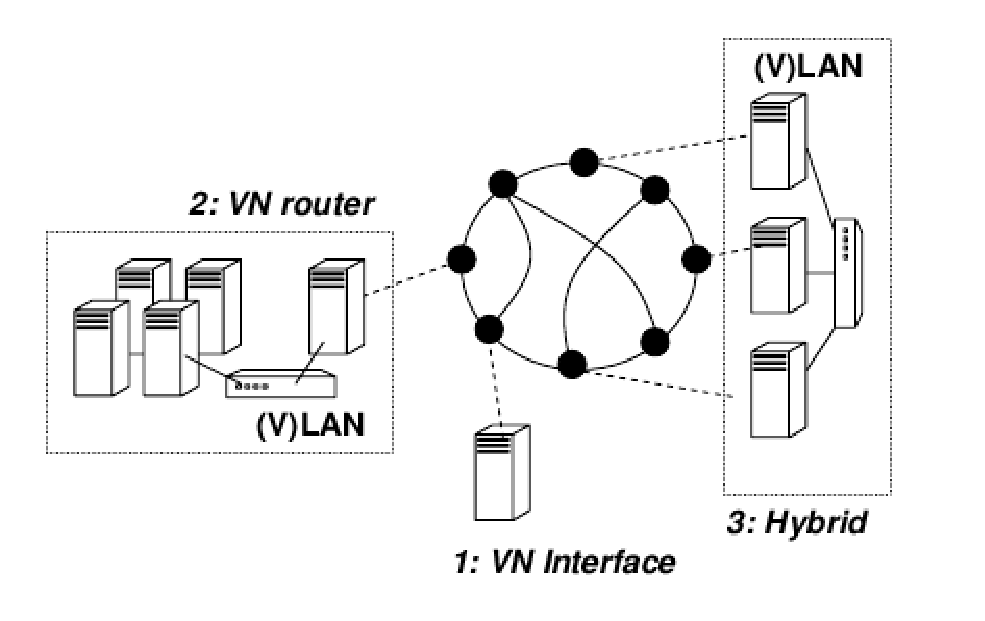
\epsfig{file=figs/three_models.png.eps}
\caption[Three VN Approaches]{Illustration of the three different deployment
models considered in this paper. In VN interface mode (1), each node has an
overlay ID and communicates to all other nodes through VN tunneling. In VN
router mode (2), only the router has an overlay ID and routes for a set of
resources; LAN communication does not require VN tunneling. In hybrid mode
(3), each host has an overlay ID; LAN communication does not require VN
tunneling.}
\label{fig:three_models}
\end{figure}

\begin{table}[ht]
\caption{Qualitative comparison of the three deployment models}
\label{tab:three_models}
\centering
\begin{tabular}{|p{1in}||p{1.25in}|p{1.5in}|p{2.25in}|} \hline
 & Interface & Router & Hybrid \\ \hline\hline
Host LAN 
& 
No assumption 
& 
Ideally, VLAN
&
No assumption, though may have duplicate address allocation in the same subnet
for different namespaces.\footnotemark[2]
\\ \hline
Host software
&
IPOP, tap
&
End node: none. Router: IPOP, tap, bridge 
&
IPOP, tap, VETH, bridge \\ \hline
Host overhead
&
CPU, memory
& 
End node: none. Router: CPU, memory
&
CPU, memory \\ \hline
LAN traffic
&
Through IPOP
&
\multicolumn{2}{c|}{Bypasses IPOP} \\ \hline
Migration
&
Handled by node
&
Involves source and target routers
&
Handled by node \\ \hline
Tolerance to faults
&
Nodes are independent
&
Router fault affects all LAN nodes
&
Nodes are independent \\ \hline
\end{tabular}
\end{table}

\begin{figure}[ht]
\centering
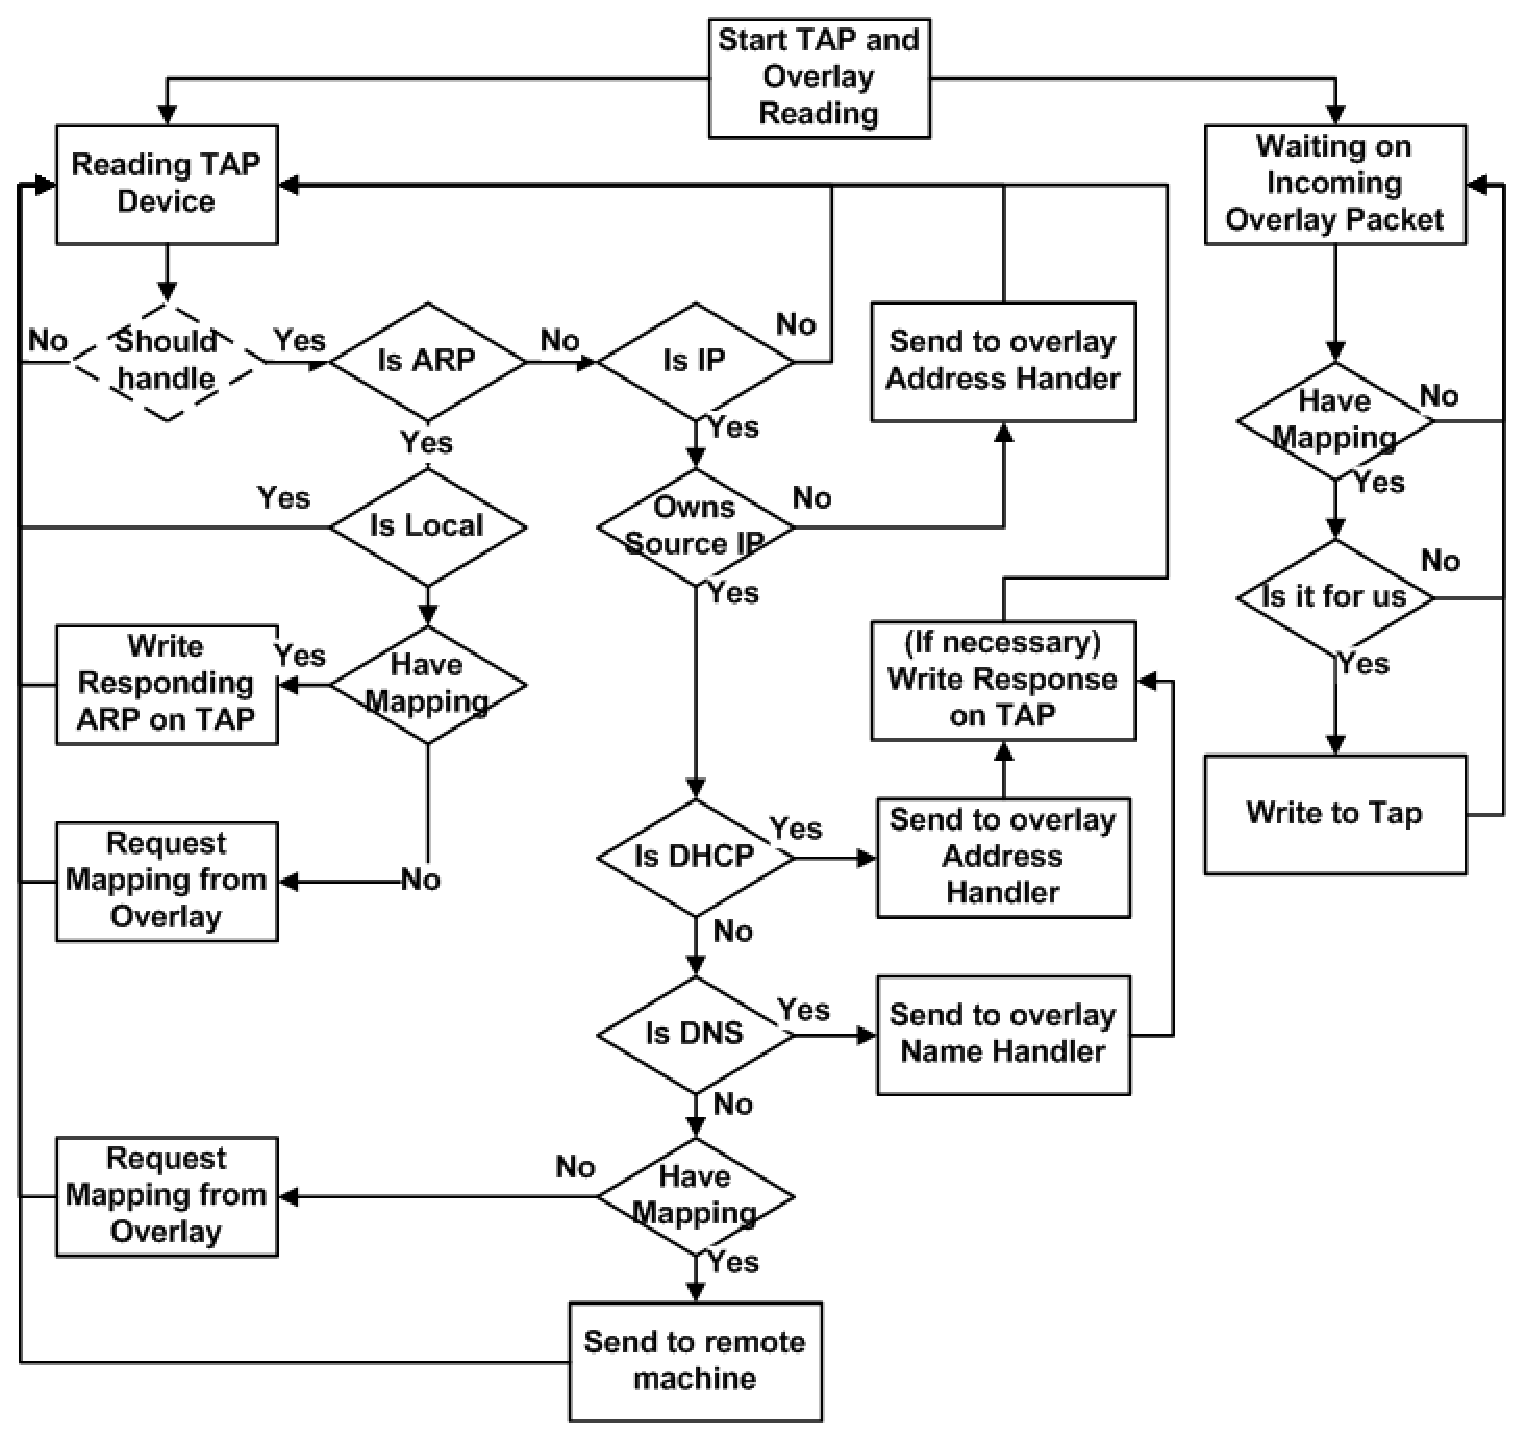
\epsfig{file=figs/vn.png.eps, width=6in}
\caption[The state diagram of a self-configuring VN.]{The state diagram of a
self-configuring VN.  In this model, a VN interface is identical to a VN router
with the caveat that the TAP device is not bridged, thus isolating the VN
traffic.  The ``Should Handle'' with dashed lines is a feature that is specific
to the VN hybrid; that is, a VN hybrid must be configured to communicate for a
single network device.}
\label{fig:vn}
\end{figure}

\begin{figure}[ht]
\centering
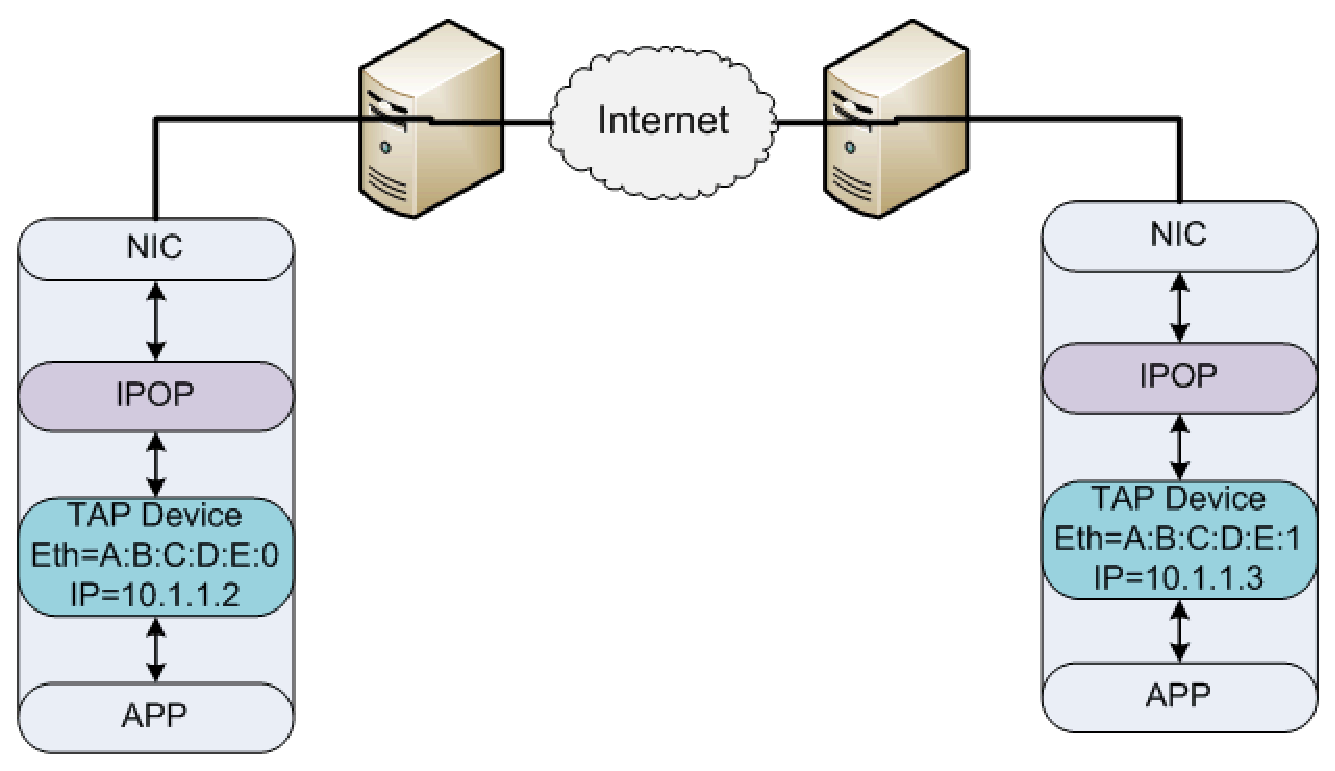
\epsfig{file=figs/tap_workstation.png.eps, width=4in}
\caption[VN Interface]{A VN deployed as an interface for single machine usage.
The user of the machine is presented two interfaces on two different IP subnets.
All non-VN subnet based traffic is routed normally via the default interface.}
\label{fig:interface}
\end{figure}

\begin{figure}[ht]
\centering
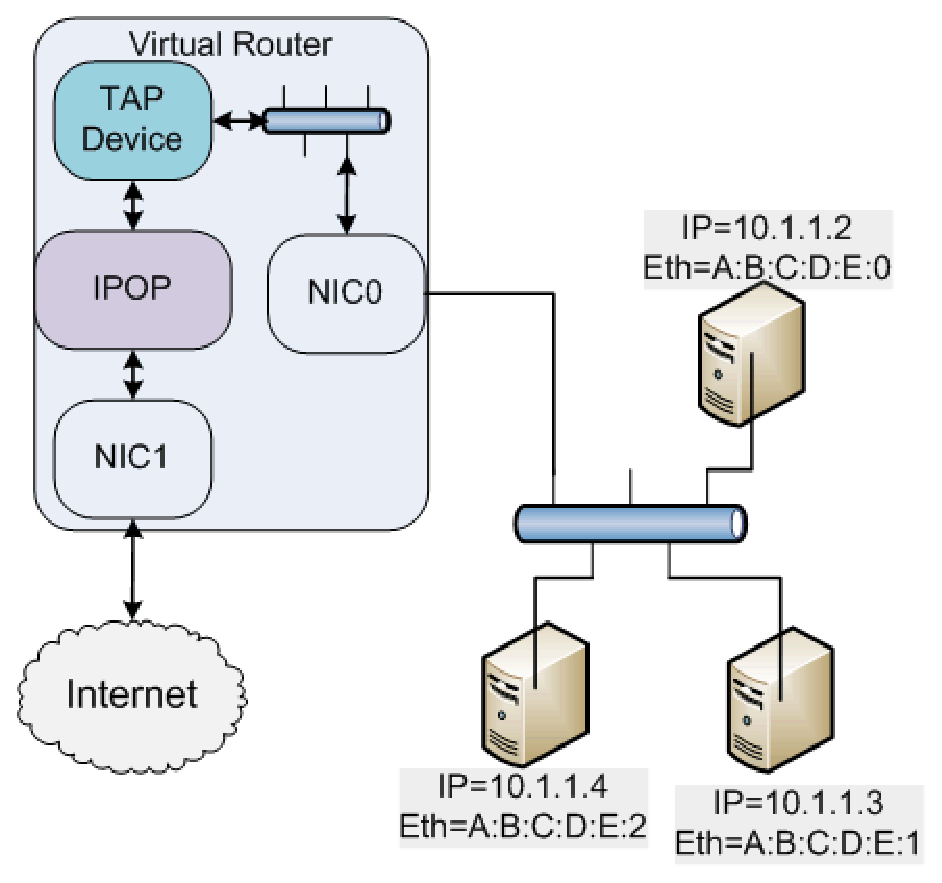
\epsfig{file=figs/tap_cluster.png.eps, width=4in}
\caption[VN Router]{A VN deployed as a router providing virtual network access
for an entire layer 2 network.  Each machine in the network only has a VN-based
address, though they can communicate directly with each other (and with proper
routing rules and NAT setup the Internet as well).  The machine hosting the VN
can also have an IP address in the network by assigning one to the bridge.}
\label{fig:router}
\end{figure}

\begin{figure}[ht]
\centering
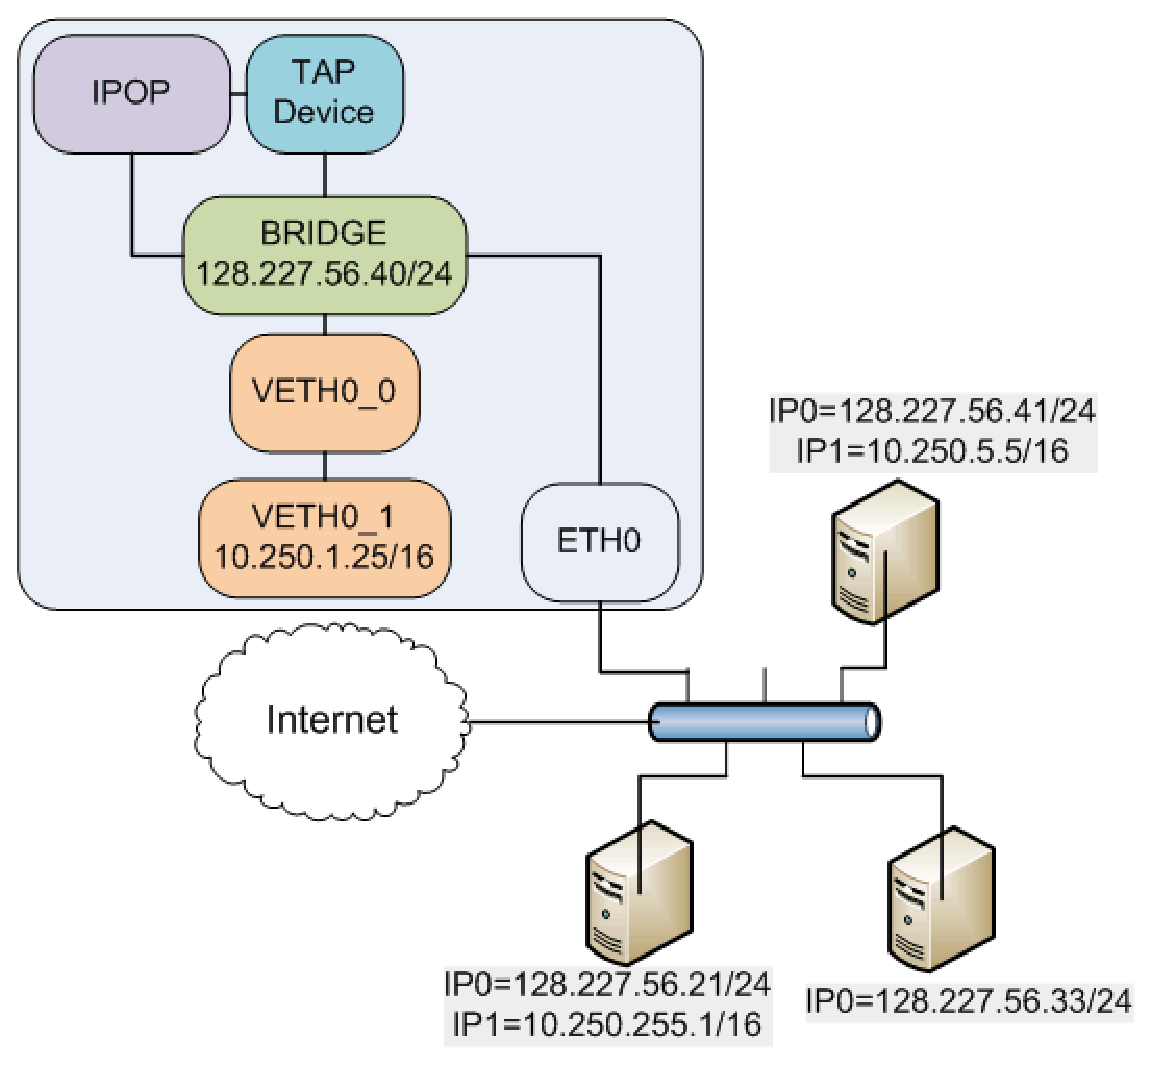
\epsfig{file=figs/tap_hybrid.png.eps, width=4in}
\caption[VN Hybrid]{A VN deployed in a hybrid mode providing virtual network
access for a single machine but bypassing the VN when a VN peer is local.  This
model is similar to having two network cards from a single machine going to one
switch.  The key feature is that this model allows a machine to be in multiple
IP address space subnets and have layer 2 traffic as well.}
\label{fig:hybrid}
\end{figure}

\begin{figure}[ht]
\centering
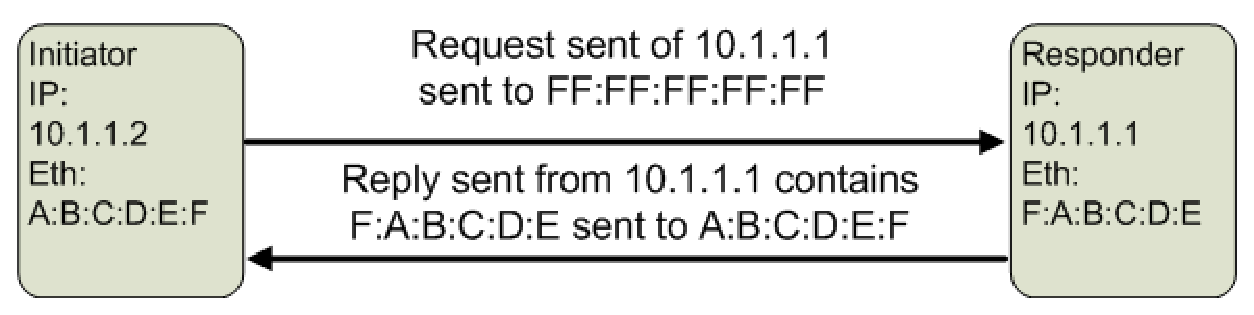
\epsfig{file=figs/arp.png.eps, width=4in}
\caption{ARP Request/Reply Interaction.}
\label{fig:arp}
\end{figure}

\begin{figure}[ht]
\centering
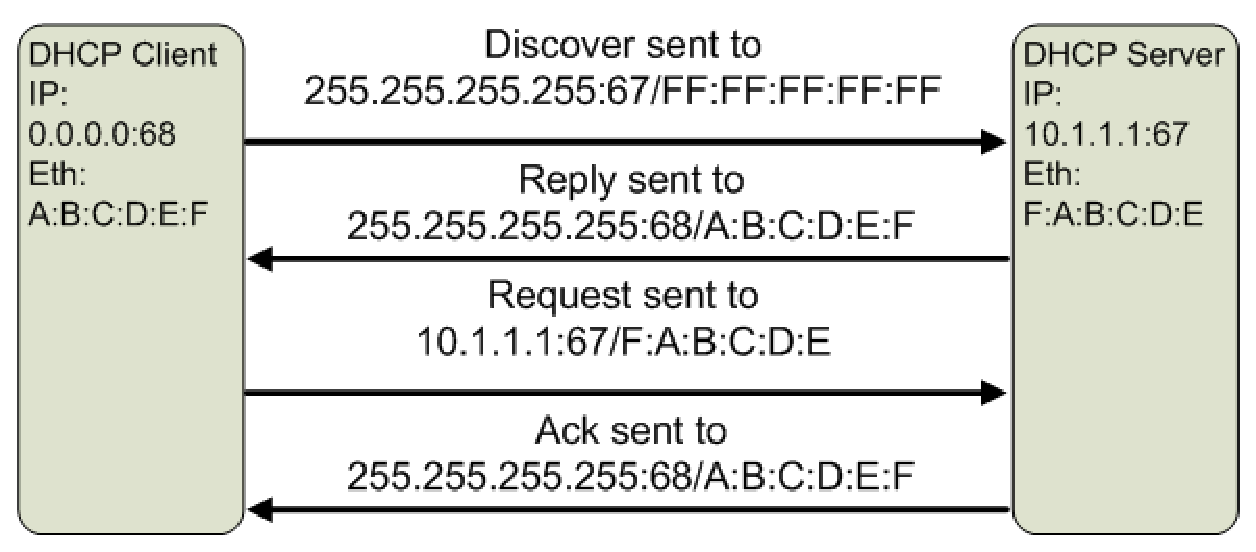
\epsfig{file=figs/dhcp.png.eps, width=4in}
\caption{DHCP Client/Server Interaction.}
\label{fig:dhcp}
\end{figure}

\begin{figure}[ht]
\centering
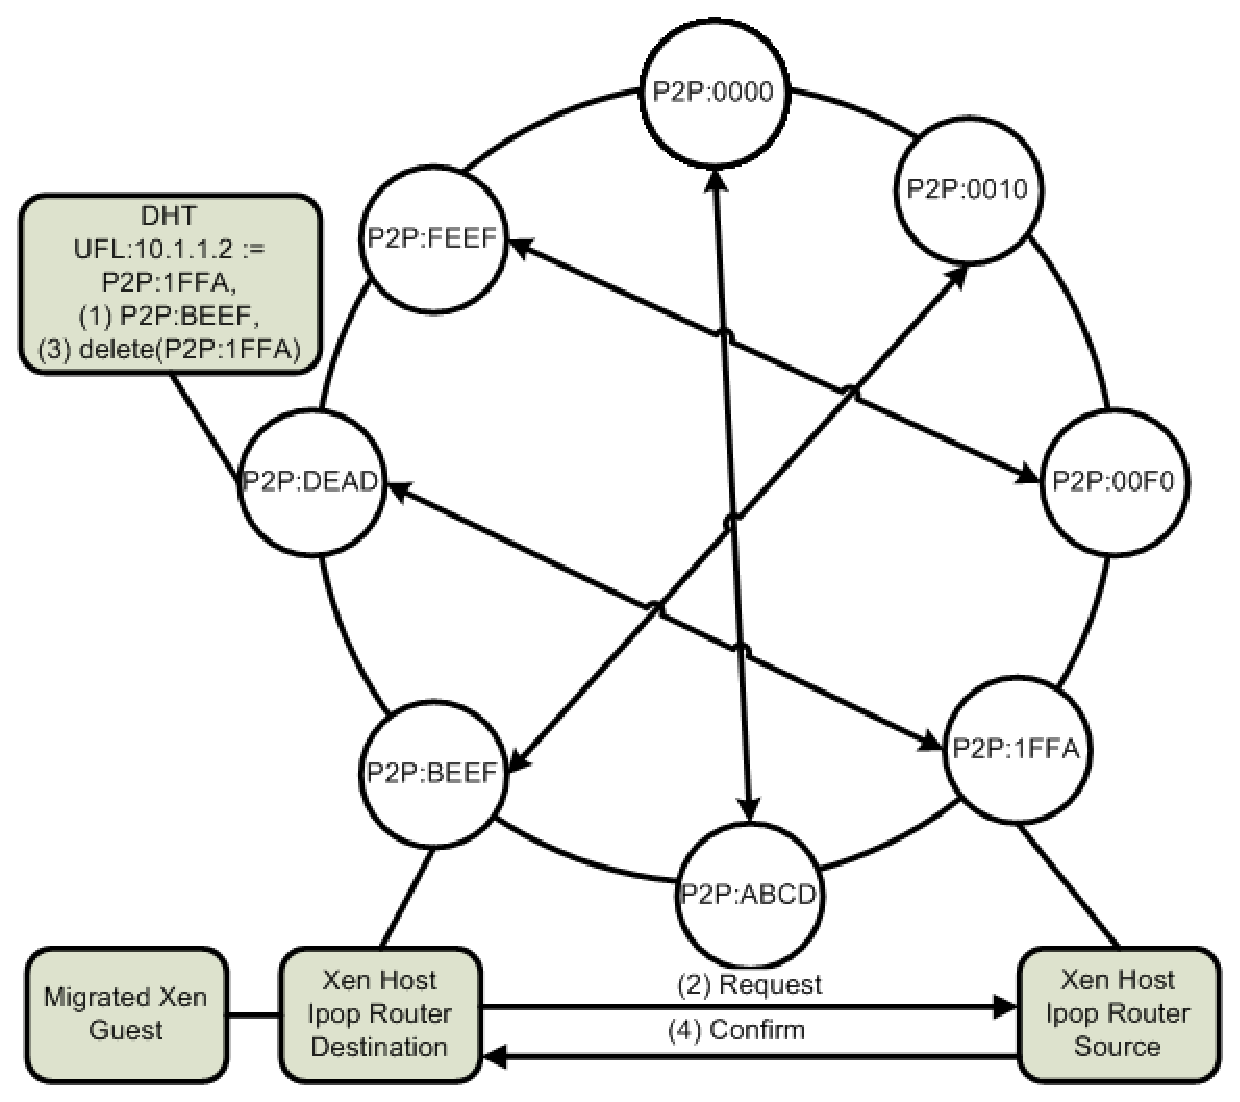
\epsfig{file=figs/Migration.png.eps, width=5in}
\caption[VN Router Migration]{The VN operations that occur after a guest (VM)
has been migrated.  (1) The destination retrieves the P2P information of the
source from the DHT and optimistically places its information into the DHT.
(2) The destination requests that the source delete its information from the
DHT.  (3)  The source confirms that the VM is no longer present and performs
the delete.  (4)  The source notifies the destination that its request has
finished successfully.}
\label{fig:migration_ring}
\end{figure}

\begin{figure}[ht]
\centering
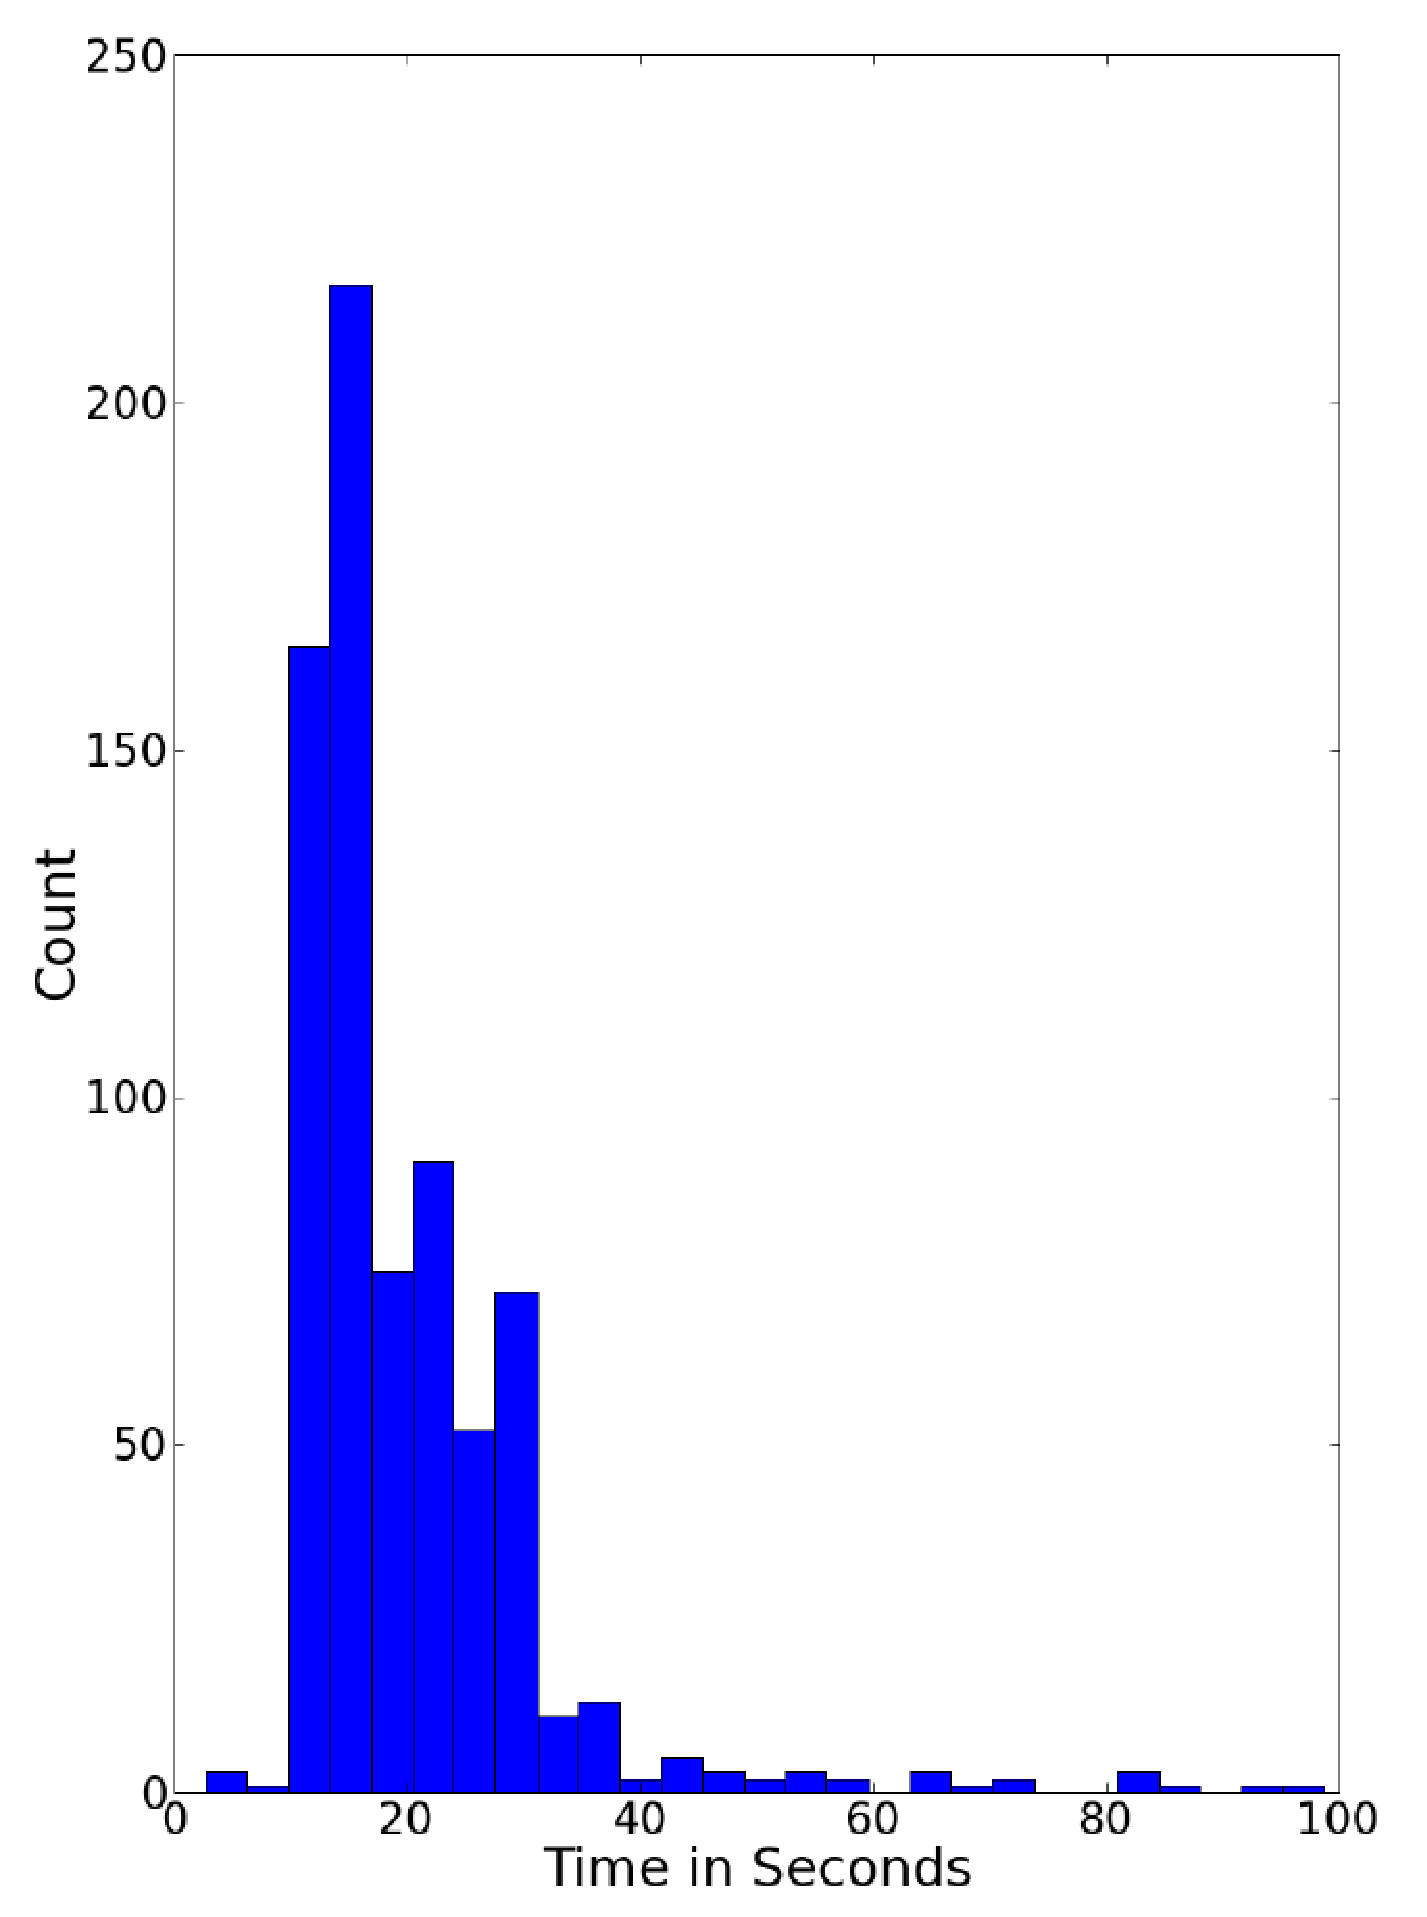
\epsfig{file=figs/migration_results.png.eps, width=2.5in}
\caption[VN Router migration evaluation]{VN Router migration evaluation.  Over
50 different IPs migrated about 10 times each.  The average was 20.11 seconds
with a standard deviation of 10.89.  In this experiment, the majority of this
time comes from VN migration, whereas VM migration requires less than a second.}
\label{fig:mig}
\end{figure}

\begin{figure}[ht]
\centering
\caption{Comparison of IP Broadcast and Multicast using overlay Broadcast and
Unicast.}
\label{fig:broadcast}
\end{figure}

\begin{figure}[ht]
\centering
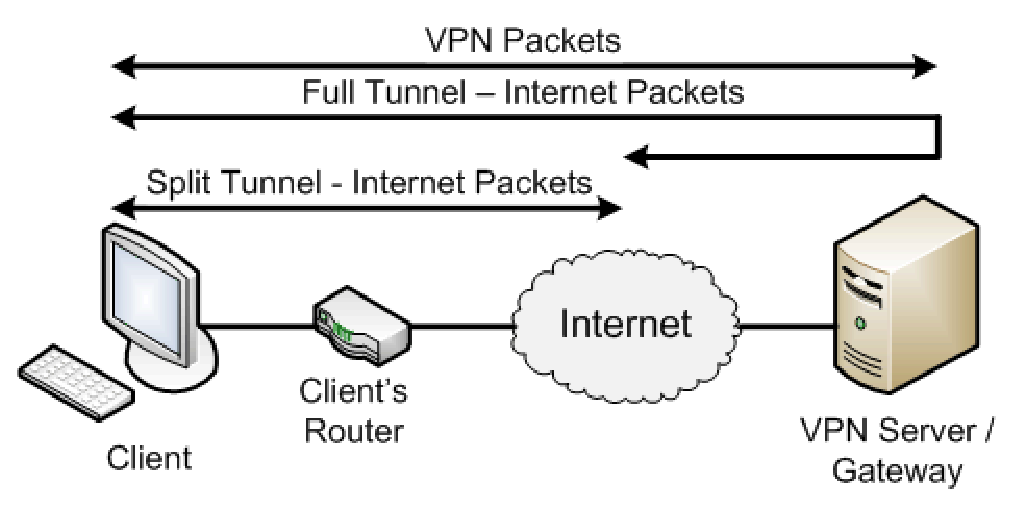
\epsfig{file=figs/tunnel.png.eps, width=4in}
\caption[An example of both full and split tunnel VPN modes]{An example of both
full and split tunnel VPN modes.  In both, packets for the server are sent
directly to the server.  In split tunnel mode, Internet packets bypass the VPN
and are routed directly to the Internet.  In full tunnel mode, Internet packets
are first routed to the VPN gateway, and then to their Internet destination.}
\label{fig:tunnel}
\end{figure}

\begin{figure}[ht]
\centering
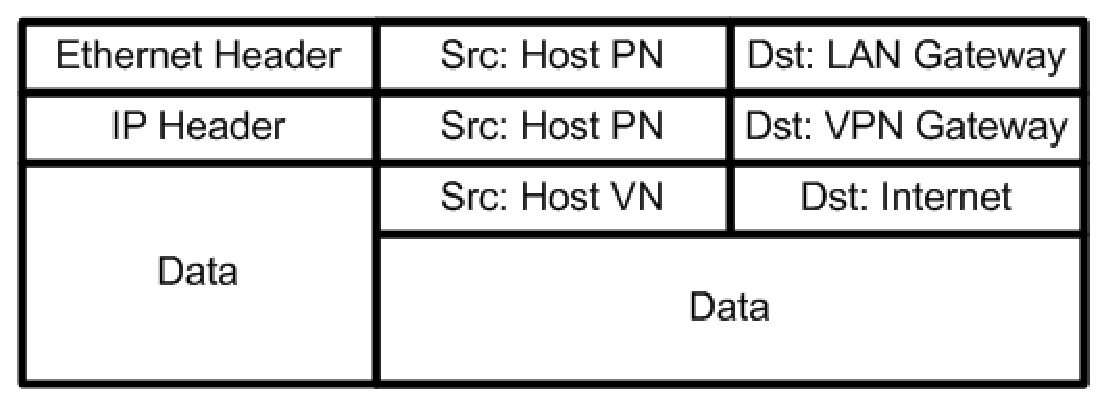
\epsfig{file=figs/tunnel_packet.png.eps, width=4in}
\caption[The contents of a full tunnel Ethernet packet]{The contents of a full
tunnel Ethernet packet.  PN and VN are defined as physical and virtual network,
respectively.}
\label{fig:tunnel_packet}
\end{figure}

\begin{table}[ht]
\centering
\begin{tabular}{|c||c|c|c|} \hline
& Google & GW Pri & GW Pub \\ \hline \hline
Ethernet & 70.6 & 12.9 & 13.9 \\ \hline
Routing & 71.4 & 13.2 & 11.0 \\ \hline
None & 66.1 & N/A & 10.9 \\ \hline
\end{tabular}
\caption[Full tunnel evaluation]{Latency results comparing full tunnel
approaches measured in ms.  Legend: GW Pri - gateway's VPN address, GW Pub -
gateway's VPN address, Ethernet - full tunnel Ethernet packet method, Routing -
full tunnel routing rule switch, None - split tunnel or no VPN.}
\label{tab:full_tunnel_eval}
\end{table}

\clearpage

\begin{figure}[ht]
\centering
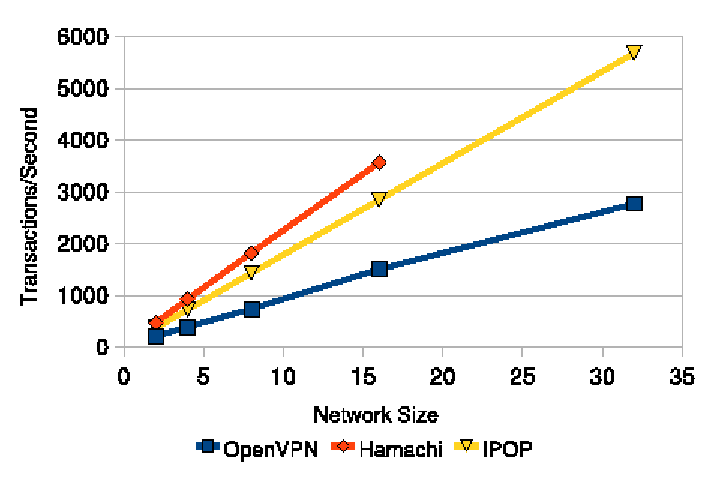
\epsfig{file=figs/latency.eps, width=4in}
\caption{System transaction rate for various VPN approaches.}
\label{fig:latency}
\end{figure}

\begin{figure}[ht]
\centering
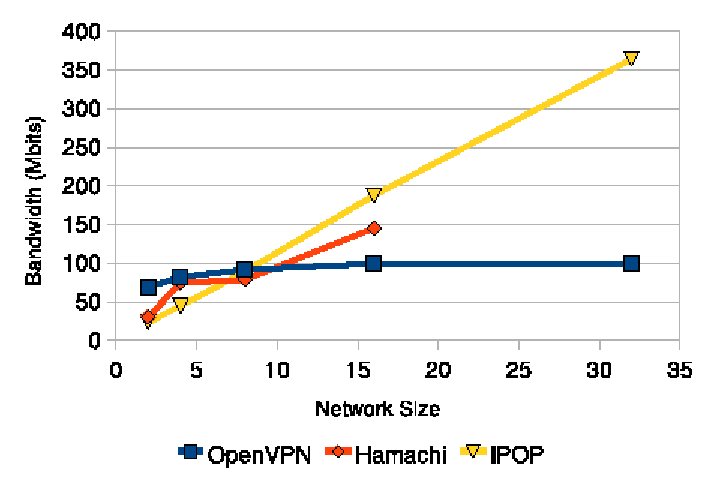
\epsfig{file=figs/bandwidth.eps, width=4in}
\caption{System bandwidth for various VPN approaches.}
\label{fig:bandwidth}
\end{figure}

\begin{figure}[ht]
\centering
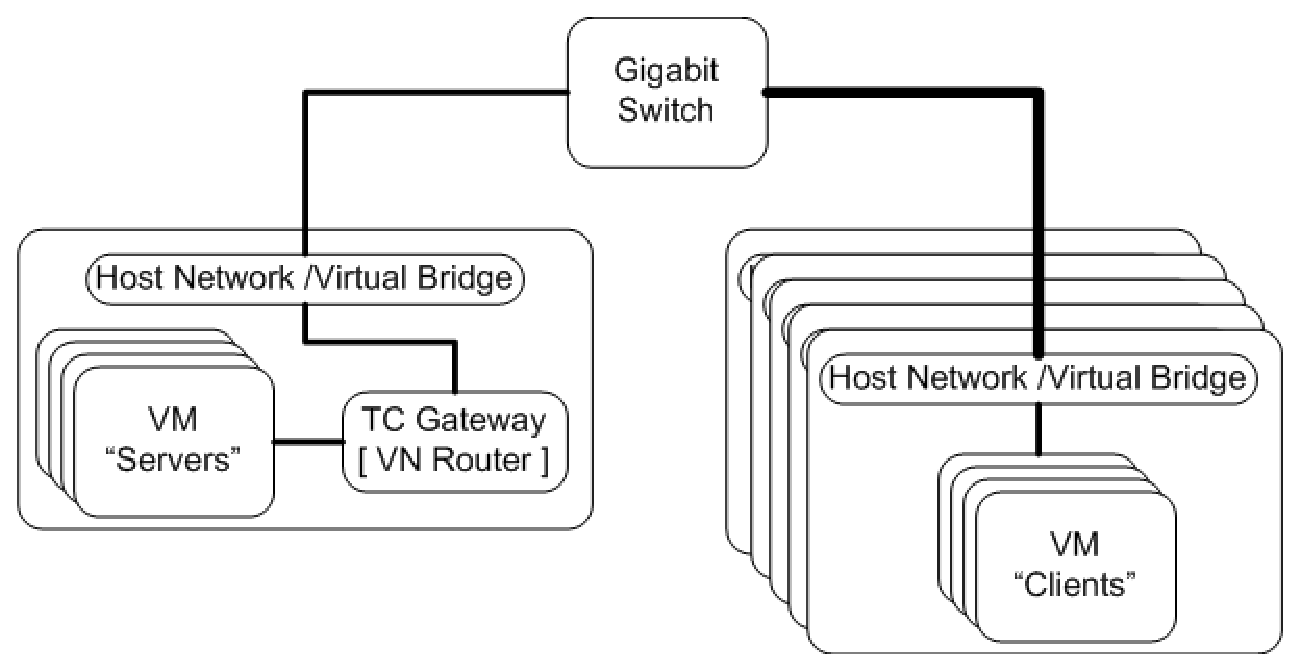
\epsfig{file=figs/grid_setup.png.eps, width=4in}
\caption[Grid evaluation setup]{The system setup for the grid experiments.  The
VM ``Servers'' ran SPECjbb and were also the site for the collection of the
netperf benchmarks.  All the VM ``Servers'' were connected through the TC
Gateway through host-only networking to the VM ``Clients''.  All traffic for
the VM ``Servers'' passes through the TC Gateway, which also doubled as the
Router in the Router experiments.}
\label{fig:gridsetup}
\end{figure}

\begin{figure}[ht]
\centering

\mbox{
\subfigure[TCP Stream bandwidth, SPECJbb load] {
  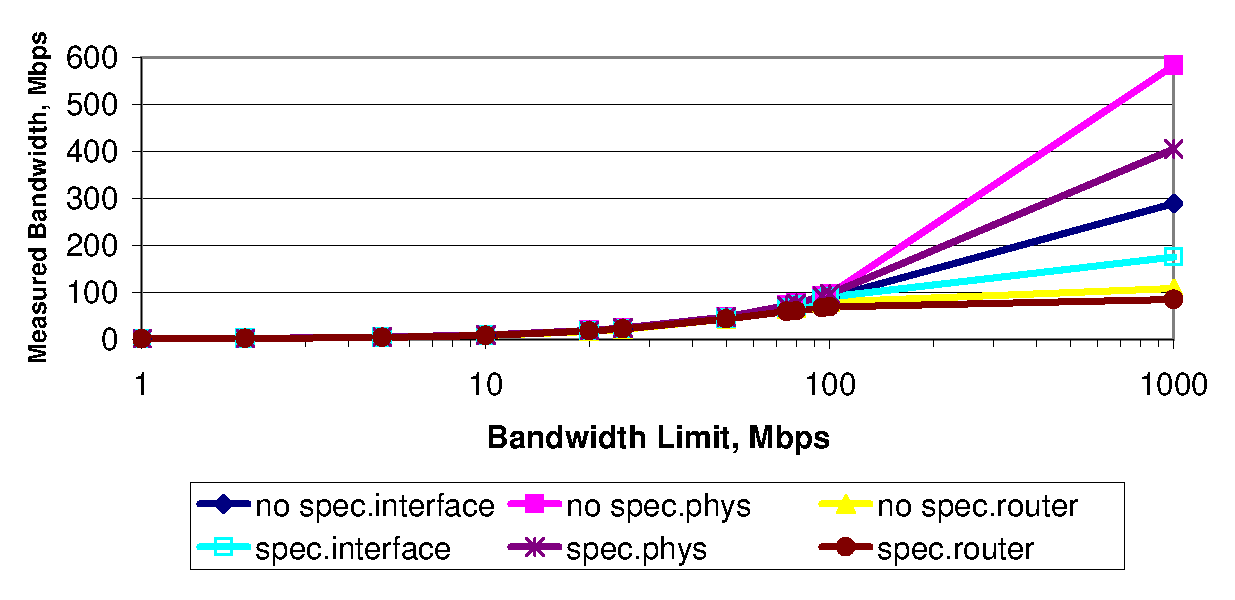
\includegraphics[width=.45\linewidth]{figs/stream.netperf.jpg.eps}
  \label{fig:stream.netperf}
}

\subfigure[TCP RR latency, SPECJbb load] {
  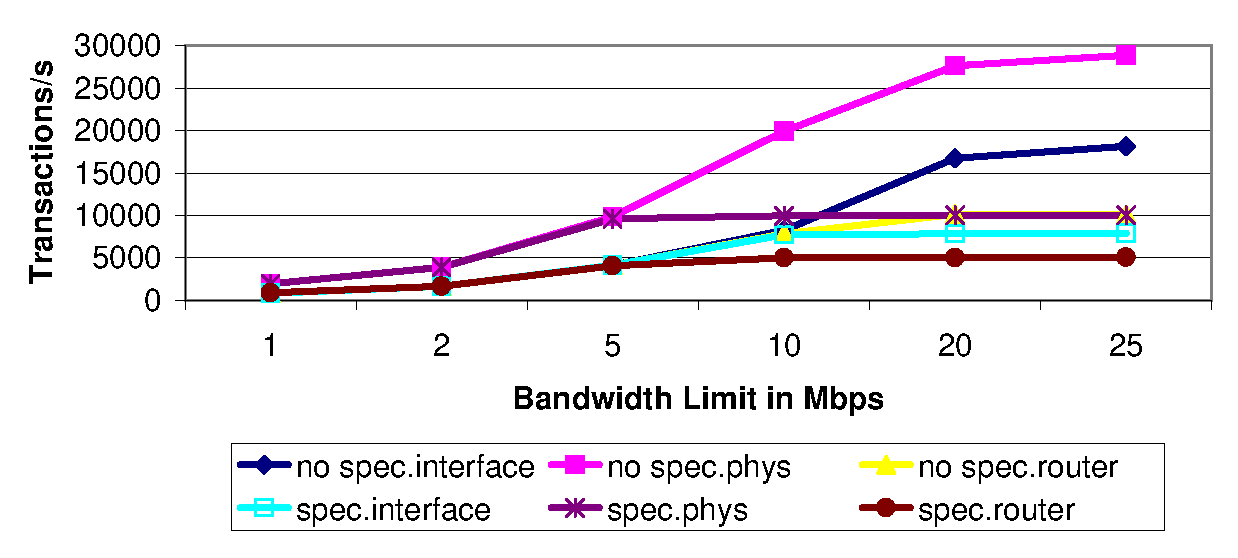
\includegraphics[width=.45\linewidth]{figs/rr.netperf.jpg.eps}
  \label{fig:rr.netperf}
}
}

\caption[Grid Netperf evaluation]{Netperf measurements with and without SPECjbb
load.  Lines are of the form (no spec, spec).(phys, interface, router).  Where
``spec'' indicates SPECjbb benchmark is active, while ``no spec'' indicates
that SPECJbb is inactive. ``phys'' implies the absence of IPOP with benchmarks
occurring directly over the ``physical'' network card.  ``interface'' and
``router'' present the results for VN interface and router models respectively.}
\label{fig:gridevalnet}
\end{figure}

\begin{figure}[ht]
\centering

\mbox{
\subfigure[SPECJbb score, TCP Stream load] {
  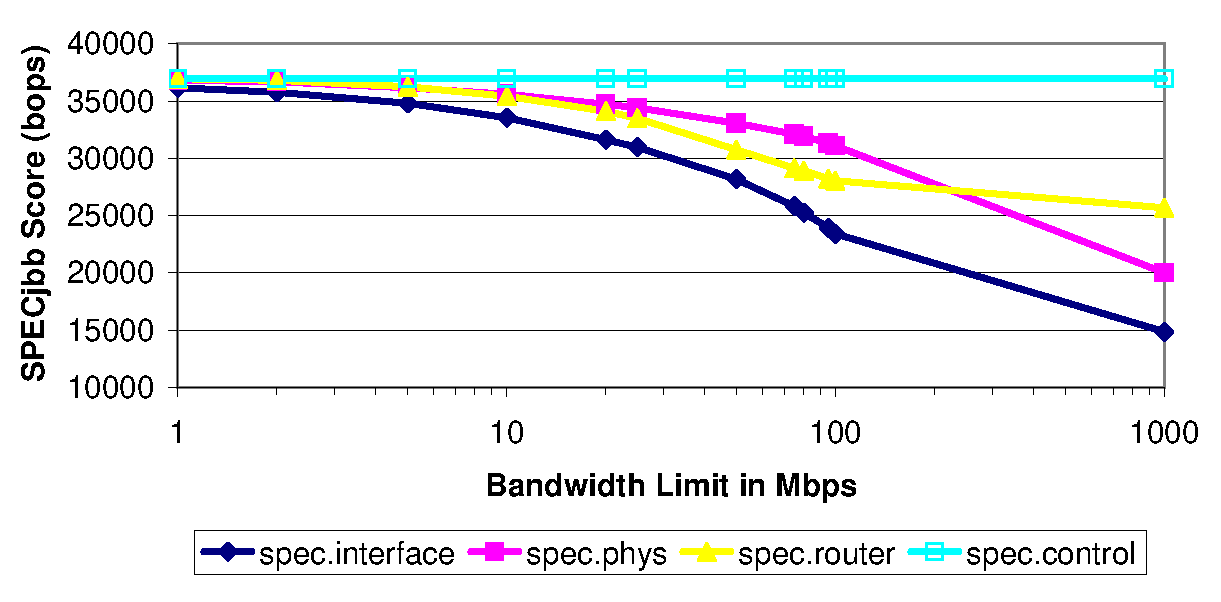
\includegraphics[width=.45\linewidth]{figs/stream.spec.jpg.eps}
  \label{fig:stream.spec}
}

\subfigure[SPECJbb score, TCP RR load] {
  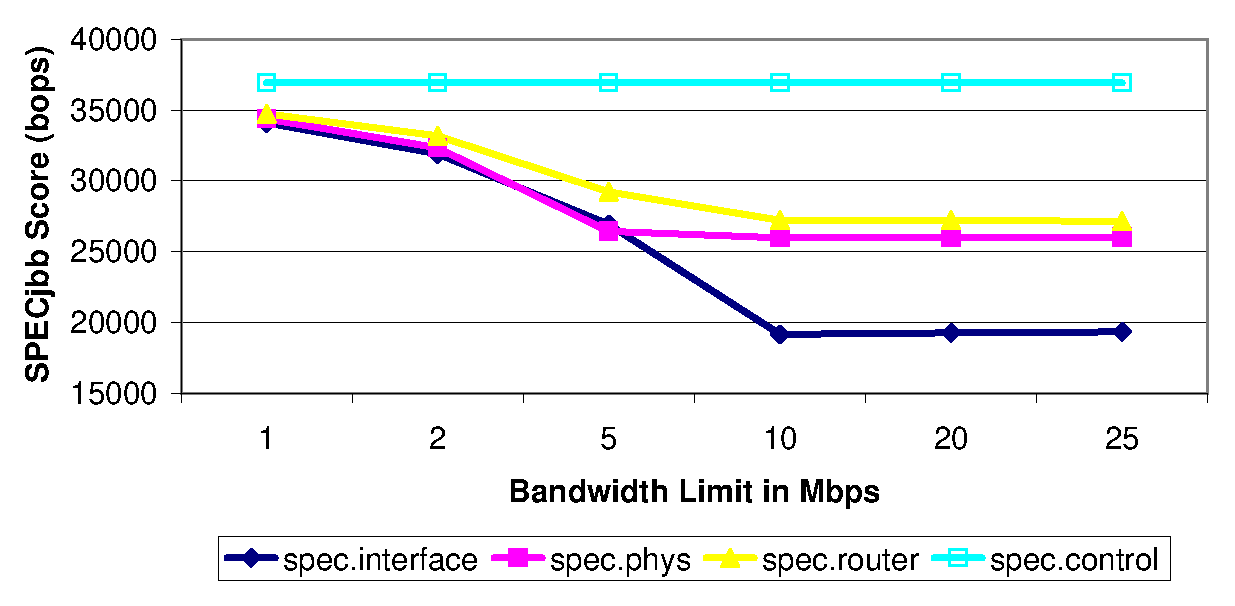
\includegraphics[width=.45\linewidth]{figs/rr.spec.jpg.eps}
  \label{fig:rr.spec}
}
}
\caption[Grid SPECjbb evaluation]{SPECjbb scores with and without Netperf load.
Lines are of the form spec.(control, phys, interface, router).  ``spec''
implies that SPECJbb executes in all tests.  In ``control'' Netperf is
inactive, that is, it is the maximum attainable value for SPECJbb. ``phys''
implies the absence of IPOP with benchmarks occurring directly over the
``physical'' network card.  ``interface'' and ``router'' present the results
for VN interface and router models respectively.}
\label{fig:gridevalcpu}
\end{figure}

\begin{table}
\centering
\begin{tabular}[c]{|l||c|c|c|} \hline
& EC2 / UF & EC2 / GoGrid & UF / GoGrid \\ \hline
Stream Phys & 89.21 & 35.93 & 30.17\\ \hline
Stream VN & 75.31 & 19.21 & 25.65\\ \hline
RR Phys & 13.35 & 11.09  & 9.97 \\ \hline
RR VN & 13.33 & 10.69 & 9.76 \\ \hline
\end{tabular}
\caption[WAN Results for inter-cloud networking]{WAN Results for inter-cloud
networking.  Stream is in Mbs and RR is in trans/s (The inverse of trans/s
would be equal to the average latency).}
\label{tab:cloud-wan}
\end{table}

\begin{table}
\centering
\begin{tabular}{|l||c|c|c|c|} \hline
 & VN Interface & VN Router & VN Hybrid & Physical \\ \hline
Stream & 109 & 325 & 324 & 327 \\ \hline
RR & 1863 & 2277 & 2253 & 3121 \\ \hline
\end{tabular}
\caption[LAN results performed at GoGrid]{LAN results performed at GoGrid.
Stream is in Mbs and RR is in trans/s.  Interface and Physical used the eth0
NIC, while Router and Hybrid used eth1.  Different VLANs may give different
results.}
\label{tab:cloud-lan}
\end{table}
